\documentclass[11pt,letter,subeqn,fleqn]{article}
%\usepackage[normalem]{ulem}
\usepackage{amsmath, amssymb,amsthm,cite}
%\usepackage[dvips]{graphics}
\usepackage[usenames,dvipsnames]{color}
%\usepackage[normal]{subfigure}
%\usepackage{subfig}
\usepackage{graphicx,subfigure}
\usepackage{tabulary}
\usepackage{float}
\usepackage{gensymb}
\usepackage{authblk}
%\usepackage{caption}
%\usepackage{subcaption}
\usepackage{geometry}

\title{Global Optimization of the Mean First Passage Time for Narrow Capture Problems in Elliptic Domains}

\author[1]{Jason Gilbert \thanks{Electronic mail: jtg074@mail.usask.ca}}
\author[1]{Alexei Cheviakov\thanks{Corresponding Author. Alternative English spelling: Alexey Shevyakov. Electronic mail: alexei.cheviakov@usask.ca}}
\affil[1]{Department of Mathematics and Statistics, University of Saskatchewan}



\setlength{\textwidth}{160.0mm} \setlength{\textheight}{240.0mm}
\setlength{\oddsidemargin}{6mm} \setlength{\evensidemargin}{0mm}
\setlength{\topmargin}{-28mm} \setlength{\parindent}{5.0mm} \setlength{\parskip}{1.0mm}


\tolerance=9999

\def \dfracskip{2ex}

\def\beq{\begin{equation}}
\def\eeq{\end{equation}}
\def\barr{\begin{array}{ll}}
\def\earr{\end{array}}
\def\eps{\varepsilon}

\def\sg#1{{\rm #1}}
\def\const{\hbox{\rm const}}
\def\diag{\hbox{\rm diag}}
\def\mod{\hbox{\rm mod}}
\def\rank{\mathop{\hbox{\rm rank}}}
\def\Image{\mathop{\hbox{\rm Image}}}
\def\mes{\mathop{\hbox{\rm mes}}}
%\def\grad{\mathop{\hbox{\rm grad}}}
\def\sign{\mathop{\hbox{\rm sign}}}
\def\ind{\mathop{\hbox{\rm ind}}}
\def\id{\mathop{\hbox{\rm id}}}
\def\d{\mathop{\hbox{\rm d}}}
\def\ad{\hbox{ad}}
\def\ch{\mathop{\hbox{\rm ch}}}
\def\th{\mathop{\hbox{\rm th}}}
\def\cth{\mathop{\hbox{\rm cth}}}
\def\sh{\mathop{\hbox{\rm sh}}}
\def\max{\mathop{\hbox{\rm max}}}
\def\ind{\mathop{\hbox{\rm ind}}}
\def\Tr{\mathop{\hbox{\rm Tr}}}
\def\grad{{\hbox{\rm grad}}}
\def\div{{\hbox{\rm div}}}
\def\Div{\mathop{\hbox{\rm Div}}}
\def\curl{\mathop{\hbox{\rm curl}}}
\def\sn{\mathop{\hbox{\rm sn}}}
\def\sech{\mathop{\hbox{\rm sech}}}
%\def\vec#1{{\boldsymbol{\rm #1}}} %\def\vec#1{{\bf {#1}}}
\def\veci#1{{\boldsymbol{#1}}} %\def\vec#1{{\bf {#1}}}
\def\tens#1{{\boldsymbol{\rm #1}}} %\def\vec#1{{\bf {#1}}}
\def\p{\partial}
\def\cn{\mathop{\hbox{\rm cn}}}
\def\sn{\mathop{\hbox{\rm sn}}}
\def\dn{\mathop{\hbox{\rm dn}}}
\def\scn{\mathop{\hbox{\footnotesize\rm cn}}}
\def\ssn{\mathop{\hbox{\footnotesize\rm sn}}}
\def\sdn{\mathop{\hbox{\footnotesize \rm dn}}}
\def\vec#1{{\boldsymbol{\rm #1}}} %\def\vec#1{{\bf {#1}}}
\def\tens#1{{\boldsymbol{\rm #1}}} %\def\vec#1{{\bf {#1}}}



%%% One Parameter %%%
\newcommand{\norm}[1]{\|{#1}\|}

%%% Two Parameters %%%
\newcommand\der[2][]{\ensuremath{\frac{d#1}{d#2}}}
\newcommand\pder[2][]{\ensuremath{\dfrac{\partial #1}{\partial #2}}}
\newcommand\sder[2][]{\ensuremath{\dfrac{{d}^{2}#1}{{d#2}^{2}}}}
\newcommand\spder[2][]{\ensuremath{\dfrac{{\partial}^{2}#1}{{\partial#2}^{2}}}}
\newcommand\tpder[2][]{\ensuremath{\dfrac{{\partial}^{3}#1}{{\partial#2}^{3}}}}



\newtheorem{theorem}{Theorem}
\newtheorem{theoremp}{Principal Result}
\newtheorem{lemma}{Lemma}
\newtheorem{proposition}{Proposition}
\newtheorem{corollary}{Corollary}

{\theoremstyle{definition} \newtheorem{definition}{Definition}
\newtheorem{example}{Example}
\newtheorem{remark}{Remark}
}

%\newcommand{\vspacebefore}{\raisebox{0ex}[3.8ex][0ex]{\null}}
\newcommand{\vspacebefore}{\raisebox{0ex}[3.9ex][0ex]{\null}}


\newcounter{tabnum}\setcounter{tabnum}{0}
\renewcommand{\thefootnote}{\alph{footnote})}


\newcommand{\boldsig}{\mbox{\mathversion{bold}$\sigma$}}
\newcommand{\boldphi}{\mbox{\mathversion{bold}$\phi$}}

\newcommand{\boldsigma}{\mbox{\mathversion{bold}$\sigma$}}
%\newcommand{\boldphi}{\vec{\phi}}
\renewcommand{\div}{\mathrm{div}}
\newcommand{\D}{\mathrm{D}}
\newcommand{\E}{\mathrm{E}}
\newcommand{\R}{\mathrm{R}}
\newcommand{\X}{\mathrm{Y}}
\newcommand{\W}{\mathrm{W}}
\newcommand{\Y}{\mathrm{Y}}
\newcommand{\Z}{\mathrm{Z}}
\newcommand{\sysR}{\vec{R}}
\newcommand{\C}{\mathbf{C}}
\newcommand{\B}{\mathbf{B}}
\newcommand{\boldP}{\mathbf{P}}
\newcommand{\boldF}{\mathbf{F}}
\newcommand{\boldE}{\mathbf{E}}
\newcommand{\sgn}{\mathop{\mathrm{sgn}}}
\newcommand{\linop}{\mathrm{L}}



%\newtheorem{prop}{Proposition}[section]
%\newtheorem{thm}{Theorem}[section]
%\newtheorem{cor}{Corollary}[section]


\def\PDEs#1#2#3{{\boldsymbol{\rm #1}}\{#2\,; #3\} }
\def\PDEsr#1#2#3#4{{\bf #1^\mathrm{#2}}\{#3\,; #4\} } %superscript roman
\def\PDEsi#1#2#3#4{{\bf #1^\mathit{#2}}\{#3\,; #4\} } %superscript ital
\def\PDEssh#1{{\bf #1} } %short form- no vars


%----Jason

% My style
\newcommand{\then}{\qquad\rightarrow\qquad}
\newcommand{\s}{\qquad\qquad}
\newcommand{\ps}{\ + \ }
\newcommand{\ms}{\ - \ }
\newcommand{\es}{\ = \ }
% Derivatives
\newcommand{\dpart}[3]{ \dfrac{\partial ^{#3} #1 }{\partial #2 ^{#3}} }
\newcommand{\dfull}[3]{ \dfrac{\fulld ^{#3} #1 }{\fulld #2 ^{#3}} }
\newcommand{\fpart}[3]{ \frac{\partial ^{#3} #1}{\partial #2 ^{#3}} }
% Braced Trig Functions
\newcommand{\bsin}[1]{\sin\left( #1 \right)}	
\newcommand{\bcos}[1]{\cos\left( #1 \right)}


% NC Definition Notation
\newcommand{\subDom}{\bar{\Omega}}
% Ward Notation
\newcommand{\amfpt}{\overline{u}_0} % Average MFPT
\newcommand{\veps}{\varepsilon}     % Epsilon (trap size)
\newcommand{\greenMat}{\mathcal{G}} % Green's Matrix
\newcommand{\vecA}{\mathcal{A}}     % Size-dependent system
\newcommand{\vecE}{\textbf{e}}      % Vector of 1
\newcommand{\trapLoc}{\mathbf{x}}   % Coordinate vector
\newcommand{\domMeas}{|\Omega|}     % Area of domain
\newcommand{\etaS}{\eta_\star}      % Parameter used in atan2 calculation
\newcommand{\meritFunc}{q}          % Merit function
% My Notation
\newcommand{\ecc}{\kappa}
% Citation Notation
\newcommand{\wardTab}{2 }
%----Jason

\begin{document}


\maketitle \numberwithin{equation}{section}
\maketitle \numberwithin{remark}{section}
\numberwithin{lemma}{section}
\numberwithin{proposition}{section}


%%%%%%%%%%%%%%%%%%%%%%%%%%%%%%%  ABSTRACT  %%%%%%%%%%%%%%%%%%%%%%%%%%%%%%
\begin{abstract}

Narrow escape and narrow capture problems which describe the average times required to stop the motion of a randomly travelling particle within a domain have applications in various areas of science. While for general domains, it is known how the escape time decreases with the increase of the trap sizes, for some specific 2D and 3D domains,  higher-order asymptotic formulas have been established, providing the dependence of the escape time on the sizes and locations of the traps. Such results allow  the use of global optimization to seek trap arrangements that minimize average escape times. In a recent paper, the escape time expansion for a 2D elliptic domain was derived, providing the dependence of the average MFPT on sizes and locations of small internal traps. The goal of this work is to systematically seek global minima of MFPT for $1\leq N\leq 50$ traps, and compare the corresponding putative optimal trap arrangements for different values of the domain eccentricity.


\end{abstract}

%%%%%%%%%%%%%%%%%%%%%%%%%%%%% INTRODUCTION %%%%%%%%%%%%%%%%%%%%%%%%%%%%%%
\section{Introduction}


The narrow capture problem, as described here, concerns the average time required for a particle undergoing Brownian motion to encounter a region within the domain, referred to as a trap, which causes its motion to cease. It is mathematically defined as a Neumann-Dirichlet Poisson problem
\begin{equation} \label{eq:defPDE}
\begin{split}
& \Delta u = -\dfrac{1}{D} \ , \quad x \in \subDom \ ; \qquad
\subDom = \Omega \setminus \mathop{\cup}_{j = 1}^{N} \Omega_{\veps_j} \ ; \\[5pt]
& \partial_n u = 0 \ , \quad x \in \partial\Omega \ ; \qquad
u = 0 \ , \quad x \in \partial\Omega_{\veps_j} \ , \quad j = 1, \ldots , N \ ;
\end{split}
\end{equation}
where $\Omega\subset \mathbb{R}^n$, $n=2,3$, denotes the physical domain of the problem; $\{\Omega_{\veps_j}\}_{j = 1}^{N}$ are small volume trap domains within $\Omega$; $\subDom$ is the domain except the traps, where the motion of particles takes place, and $\partial_n$ denotes the normal derivative on the boundary of the domain. The diffusivity $D$ of the medium filling $\subDom$ is assumed constant. Problem  \eqref{eq:defPDE} describes the distribution of the mean capture time, the time $u(x)$ needed for a  particle to be captured by any trap, averaged over a large number of launches from the same point $x\in \subDom$. An illustration of the problem is provided in Figure \ref{fig:ProblemSchematic}.

\begin{figure}[H]
\centering
\subfigure[]{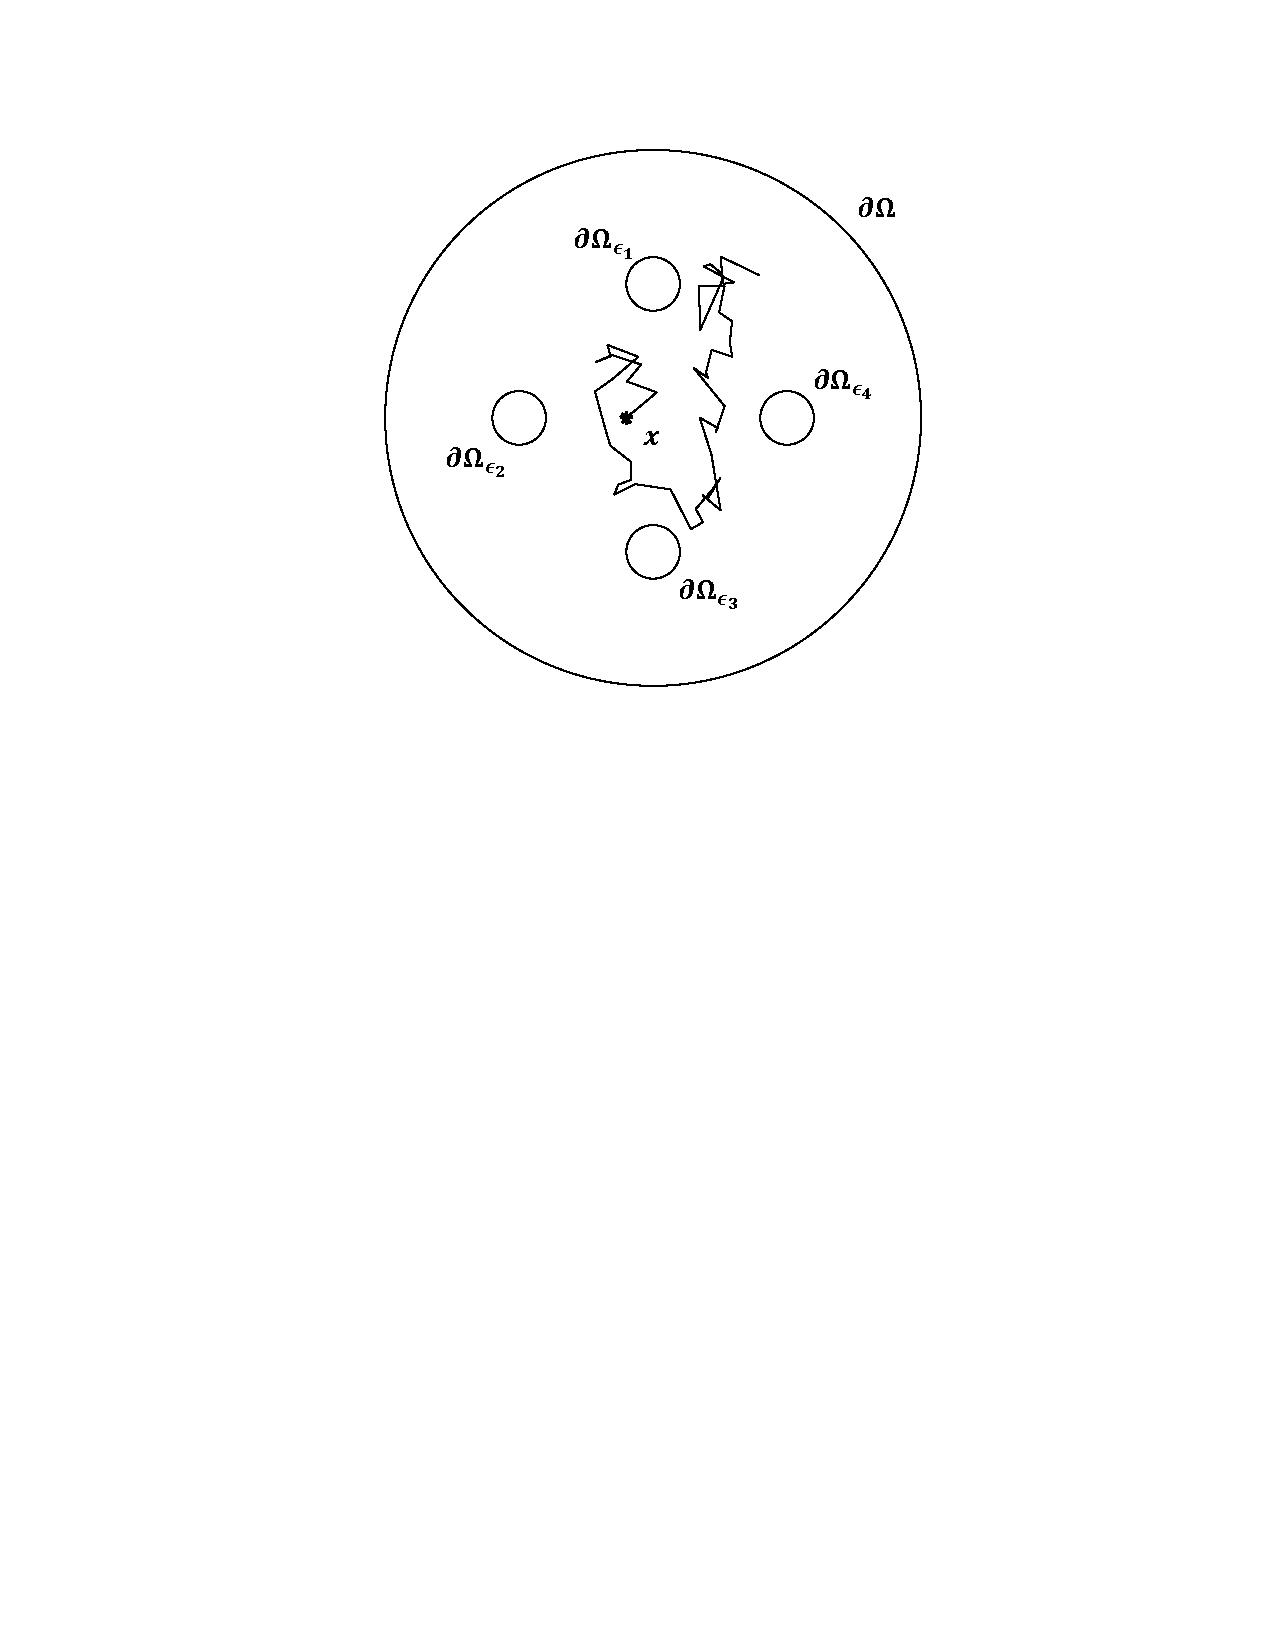
\includegraphics[width=0.3\textwidth]{ProblemSchematic2D.pdf}}
\hspace{5ex}
\subfigure[]{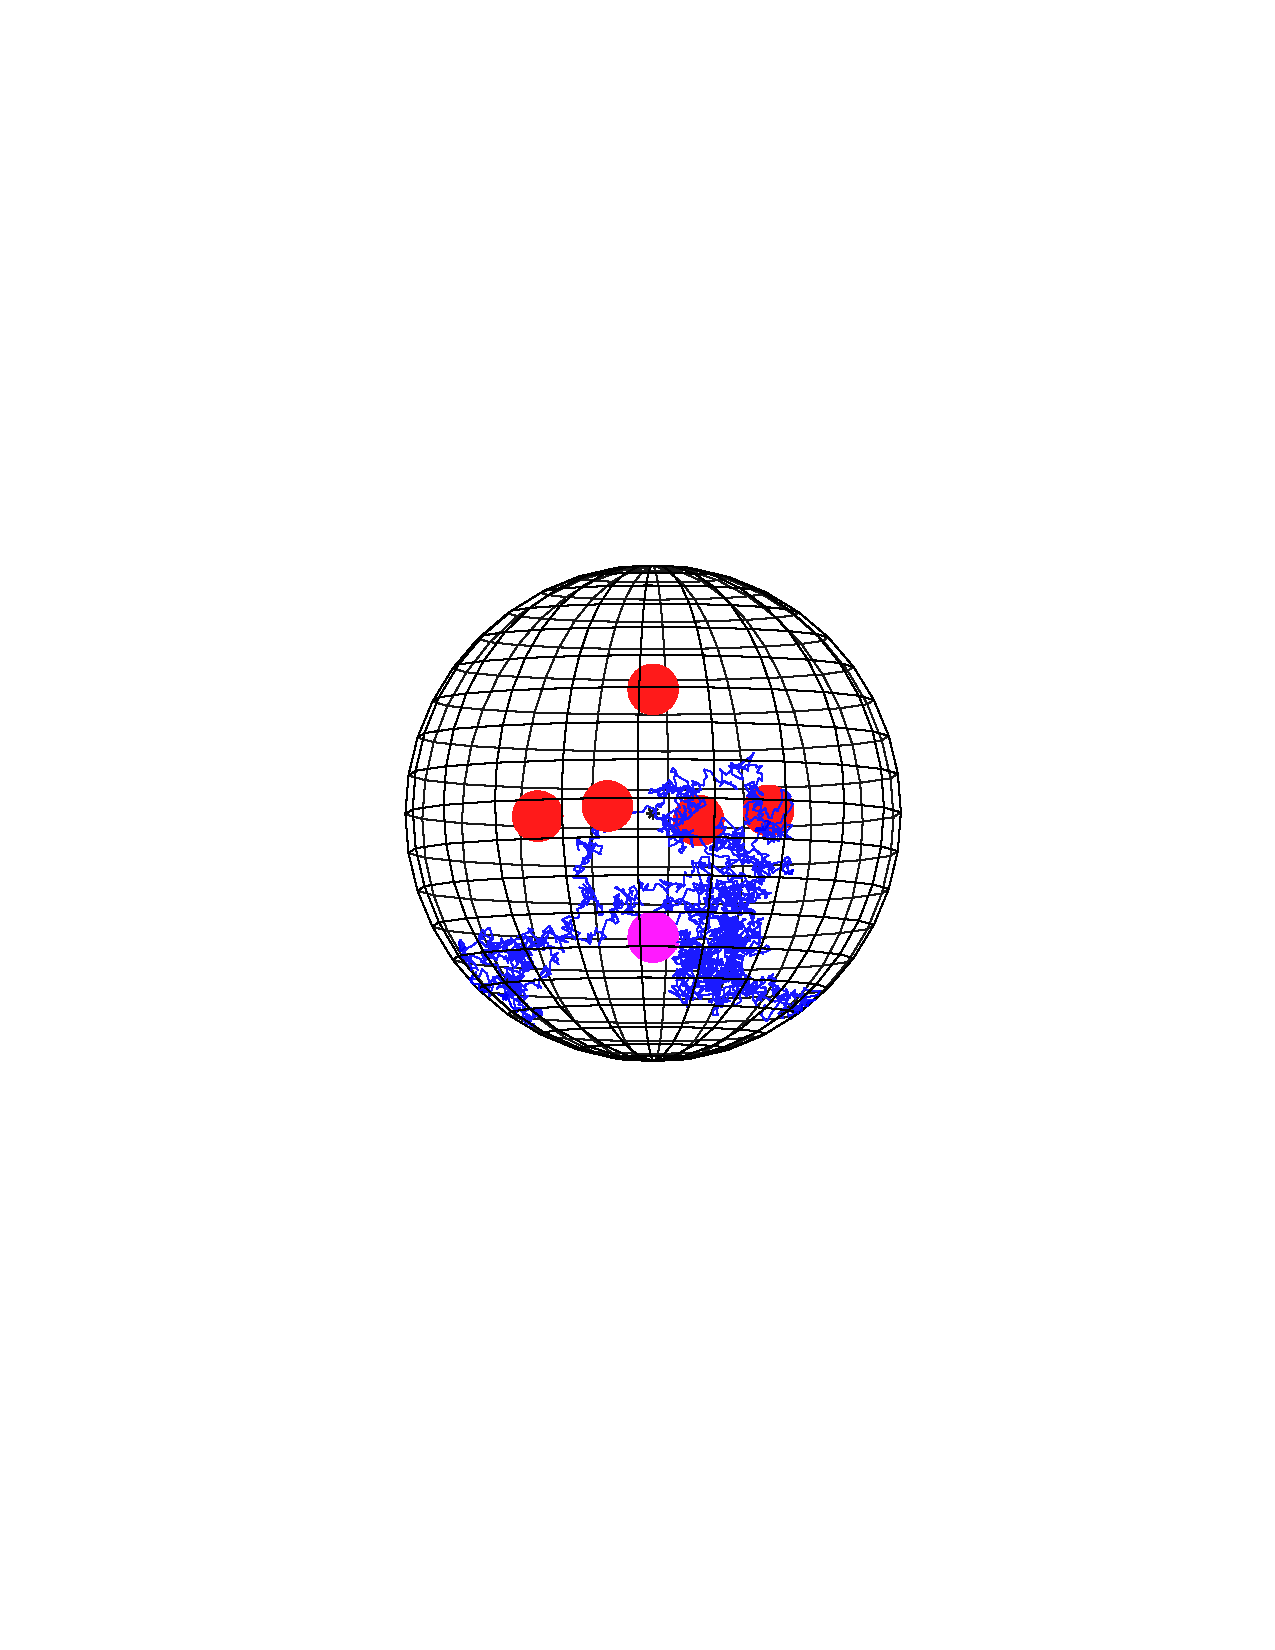
\includegraphics[width=0.3\textwidth]{ProblemSchematic3D.pdf}}
\caption{ (a) A two-dimensional narrow capture problem in the unit disk containing internal traps with absorbing boundaries $\{\partial\Omega_{\epsilon_j}\}$. (b) A three-dimensional narrow capture problem, a sample Brownian particle trajectory, leading to a capture in a trap (lowermost) denoted by purple color (color online).}
\label{fig:ProblemSchematic}
\end{figure}

The boundary conditions on $\partial \Omega$ are reflective: $\partial_n u = 0$, whereas the traps $\Omega_{\veps_j}$ are characterized by immediate absorption of a boundary particle, which is manifested by a Dirichlet boundary conditions $u = 0$ on all $\partial\Omega_{\veps_j}$.

The above generic formulation affords a variety of physical interpretations, ranging from biological to electrostatic (see, e.g., Ref.~\cite{red2001, holcman2014narrow} for an overview of applications). In this work, it will be strictly considered in terms of a particle undergoing Brownian motion \cite{saffman1975brownian}. In this case, the problem  regards the stopping time
\cite{red2001, ralf2014first}
of a Brownian particle,
confined to a domain with a reflective boundary which contains a number of absorbing ``traps". When the path of the particle intersects the boundary of one of these traps, the particle is captured, meaning that the process of Brownian motion is stopped. This stopping time may be interpreted as the time required for the particle to leave the confining domain, thus it is often referred to as the first passage time \cite{bressloff2008diffusion, bressloff2013stochastic, holcman2004escape}.
As Brownian motion is an inherently random process, there is no single first passage time which accurately characterizes the process; instead, the mean first passage time (MFPT), representing the average time taken for a particle to encounter a trap based on its first observed position, is used.
Interpreting the problem \eqref{eq:defPDE} accordingly, $u$ is the MFPT; $D$ is the diffusion coefficient, representing the mobility of the Brownian particle;  $\Omega_{\veps_j}$ is the portion of the domain occupied by the $j_{th}$ trap.

Given the physical domain and the number and sizes of the traps, it is of interest to ask whether there is an \emph{optimal} arrangement of traps within the domain which minimizes the MFPT, or in other words, maximizes the rate at which Brownian particles encounter the absorbing traps. Related work dedicated to similar optimization, in the case that the traps are asymptotically small relative to the size of the domain, for various kinds of confining domains with interior or boundary traps, can be found, for example, in Refs \cite{kolokolnikov2005optimizing, iyaniwura2020optimization, cheviakov2011optimizing, gilbert2019globally, ridgway2019locally} and references therein. Both (putative) globally optimal and multiple locally optimal arrangements of boundary and volume traps have been computed in various settings.

In this contribution, we consider the narrow capture problem for the case of a 2D elliptical domain, elaborating on previous work on the subject for the case of a circular domain \cite{kolokolnikov2005optimizing}, and the more general case of the elliptical domain \cite{iyaniwura2020optimization}.
The paper is organized as follows. In Section \ref{sec:problem} we briefly summarise the previous results which this work is based on. This includes a review of the approximations used in the case that the traps are small relative to the domain size, and are well-separated; as well as an explanation of the choice of merit function, and relevant constraints, for each case.

In Section \ref{sec:method} the optimization method chosen in our study is described. This includes an explanation of our selection of algorithms, as well the details of their use, and some decisions made to facilitate comparison to previous studies. Specifically, we seek the optimal configuration of traps for numbers of traps $N \leq 50$, and elliptic domain eccentricities of $0$, $1/8$, $1/4$, and $1/2$.

In Section \ref{sec:results} the results of the study are presented. These results include the optimized values of the merit functions (related to the domain-average Brownian particle capture time) for each number of traps, and each domain eccentricity; in the case of the unit disk, our results are compared to those of a previous study. Additionally, the distributions of traps for some illustrative cases are shown, and bulk measures of trap distribution are calculated for each of the optimized configurations.

In Section \ref{sec:discussion}, the results presented in Section \ref{sec:results} are discussed, and some remarks are provided regarding on the distribution of traps, the interpretation of the bulk quantities used, and some related problems.



\section{Problem Statement} \label{sec:problem}


The goal of this contribution is to further explore the optimal configuration of absorbing traps in terms of the asymptotic expansions for the circular and elliptical domains for which asymptotic MFPT formulae depending on trap positions are now available \cite{kolokolnikov2005optimizing, iyaniwura2020optimization}. To this end, numerical methods will be used to approximate the optimum configurations of larger numbers of traps than have previously been considered. In the case of the unit disk, the parameter space used in this study is general and does not assume any simplifying restrictions that have been imposed in previous works to reduce computation complexity.

In essence, the problem at hand is to find the trap positions which minimize the spatial average of the MFPT $u(x)$, denoted by $\amfpt$. This section will summarize the equations used to minimize this quantity, as derived in \cite{kolokolnikov2005optimizing, iyaniwura2020optimization}. Here the unit disk will be considered a special case of the elliptical domain with zero eccentricity. In either case, when the domain contains $N$ identical circular traps, each of radius $\veps$, the average MFPT satisfies \cite{iyaniwura2020optimization}
\begin{equation} \label{eq:ellAMFPT}
\amfpt \es \dfrac{\domMeas}{2\pi D\nu N} \ps \dfrac{2\pi}{N}\vecE^{T}\greenMat \vecA \ ,
\end{equation}
where the column vector $\vecA$ is the solution of the linear system
\[
\left[ I + 2\pi\nu\left( I - E \right)\greenMat \right]\vecA \es \dfrac{\domMeas}{2\pi D N}\vecE \ .
\]
Here $E \equiv \vecE\vecE^{T}/N$, $\vecE = (1, \ldots, 1)^{T}$, $\nu \equiv -1/\log\veps$, and the Green's matrix $\greenMat$ depends on the trap locations $\lbrace \trapLoc_1, \ldots , \trapLoc_N \rbrace$, such that
\begin{equation} \label{eq:ellGmat}
\greenMat_{ij} \es \left\lbrace
\begin{array}{ll}
G(\trapLoc_i ; \trapLoc_j) \quad \text{if} \ i \neq j \ , \\[5pt]
R(\trapLoc_i ; \trapLoc_j) \quad \text{if} \ i = j  \ ;
\end{array}
\quad \text{where} \quad
R(\trapLoc_i ; \trapLoc_j) = \lim_{\trapLoc_i \to \trapLoc_j} G(\trapLoc_i ; \trapLoc_j)
\right.
\end{equation}
where $G$ is the Green's function of the domain.

Examining the equation \eqref{eq:ellAMFPT}, it can be seen that the first term depends only on the combined trap size but does not depend on the trap locations. The second term explicitly depends on the trap locations is the quantity and therefore can be optimized by adjusting trap positions. The merit function subject to optimization can be chosen as
\begin{equation} \label{eq:ellMerit}
\meritFunc\left( \trapLoc \right) \es \vecE^{T}\greenMat \vecA \ .
\end{equation}
For a value of $\meritFunc$ to be a permissible solution, it is required that $\amfpt \geq 0$, as it is a measure of time; all traps must be within the domain; no trap may be in contact with any other trap (or the two must instead be represented as a single non-circular trap).

While the preceding statements are true for both the circular and the elliptical domain, the elements of the matrix $\greenMat$ are populated by evaluating the Green's function of the domain for each pair of traps, and the form of this function differs for the two cases considered here.

%\subsection{Circular Domain}
In the case of the circular domain, the elements of the Green's matrix $\greenMat$ are computed using the Neumann Green's function \cite{kolokolnikov2005optimizing}
\begin{subequations}
% Equation 4.3a
\begin{equation} \label{cirGreenFunc}
G(\trapLoc ; \trapLoc_0) \es \dfrac{1}{2\pi}\left(
-\log|\trapLoc - \trapLoc_0| \ms \log\left| \trapLoc|\trapLoc_0| - \dfrac{\trapLoc_0}{|\trapLoc_0|} \right| \ps \dfrac{1}{2}\left(|\trapLoc|^2 + |\trapLoc_0|^2\right) \ms \dfrac{3}{4}
\right) \ ,
\end{equation}
and its regular part
% Equation 4.3b
\begin{equation}
R(\trapLoc) \es \dfrac{1}{2\pi}\left(
-\log\left| \trapLoc|\trapLoc| - \dfrac{\trapLoc}{|\trapLoc|} \right| \ps |\trapLoc|^2 \ms \dfrac{3}{4}
\right) \ .
\end{equation}
\end{subequations}


%\subsection{Elliptical Domain}

The Green's function for the elliptical domain, in the form of a quickly convergent series, has been derived in \cite{iyaniwura2020optimization} using elliptical coordinates $(\xi,\eta)$. It has the form
\begin{equation} \label{eq:ellGreenFunc}
\begin{split}
G(\trapLoc, \trapLoc_0) \es \dfrac{1}{4\domMeas}\left( |\trapLoc|^2 + |\trapLoc_0|^2 \right) \ms \dfrac{3}{16\domMeas}(a^2 + b^2) \ms \dfrac{1}{4\pi}\log\beta \ms \dfrac{1}{2\pi}\xi_>  \\[5pt]
\ms \dfrac{1}{2\pi}\sum^{\infty}_{n=0}\log\left( \prod_{j=1}^{8} |1 - \beta^{2n}z_j| \right) \ ,
\qquad
\trapLoc \neq \trapLoc_0 \ ,
\end{split}
\end{equation}
where $a$ and $b$ are the major and minor axis of the domain, respectively; the area of the domain is $\domMeas = \pi ab$, the parameter $\beta = (a - b)/(a + b)$, and the values $\xi_> = \max(\xi, \xi_0)$, $z_1, \ldots, z_8$ are defined in terms of the elliptical coordinates $\xi$ and $\eta$ as follows.

The Cartesian coordinates $(x,y)$ and the elliptical coordinates $(\xi,\eta)$ are related by the transformation
\begin{subequations}
\begin{equation} \label{eq:ellCoordsA}
x = f\cosh\xi\cos\eta \ , \quad
y = f\sinh\xi\sin\eta \ , \quad
f = \sqrt{a^2 - b^2} \ .
\end{equation}
For the major and minor axis of the elliptical domain, one has
\begin{equation} \label{eq:ellCoordsB}
a = f\cosh\xi_b \ , \quad
b = f\sinh\xi_b \ , \quad
\xi_b = \tanh^{-1}\left(\dfrac{b}{a}\right) = -\dfrac{1}{2}\log\beta \ .
\end{equation}
\end{subequations}
For the backward transformation, to determine $\xi(x, y)$, equation \eqref{eq:ellCoordsA} is solved to give
\begin{subequations}
\begin{equation}
\xi = \dfrac{1}{2}\log\left( 1 - 2s + 2\sqrt{s^2 - s} \right) \ , \quad
s \equiv \dfrac{-\mu - \sqrt{\mu^2 + 4f^2y^2}}{2f^2} \ , \quad
\mu \equiv x^2 + y^2 - f^2 \ .
\end{equation}
In a similar fashion, $\eta(x, y)$ is found in terms of $\etaS \equiv \sin^{-1}(\sqrt{p})$ to be
\begin{equation}
\eta \es \left\lbrace \begin{array}{ll}
\etaS \ ,        & \text{if}\ x \geq 0,\ y \geq 0 \\[5pt]
\pi - \etaS \ ,  & \text{if}\ x < 0,\ y \geq 0 \\[5pt]
\pi + \etaS \ ,  & \text{if}\ x \leq 0,\ y < 0 \\[5pt]
2\pi - \etaS \ , & \text{if}\ x > 0,\ y < 0 \\[5pt]
\end{array}
\right. \ ,
\quad \text{where} \quad
p\equiv \dfrac{-\mu + \sqrt{\mu^2 + 4f^2y^2}}{2f^2} \ .
\end{equation}
\end{subequations}
Finally, the $z_j$-terms appearing in the infinite sum of equation \eqref{eq:ellGreenFunc} are defined via $\xi$, $\eta$, and $\xi_b$ as
\begin{equation} \label{eq:ztermsG}
\begin{array}{lll}
z_1 \equiv e^{-|\xi - \xi_0| + i(\eta - \eta_0)} \ ,          &
z_2 \equiv e^{ |\xi - \xi_0| - 4\xi_b + i(\eta - \eta_0)} \ , &
z_3 \equiv e^{-(\xi + \xi_0) - 2\xi_b + i(\eta - \eta_0)} \ , \\[4pt]
z_4 \equiv e^{ (\xi + \xi_0) - 2\xi_b + i(\eta - \eta_0)} \ , &
z_5 \equiv e^{ (\xi + \xi_0) - 4\xi_b + i(\eta + \eta_0)} \ , &
z_6 \equiv e^{-(\xi + \xi_0) + i(\eta + \eta_0)}          \ , \\[4pt]
z_7 \equiv e^{|\xi - \xi_0| - 2\xi_b + i(\eta + \eta_0)}  \ , &
z_8 \equiv e^{-|\xi - \xi_0| - 2\xi_b + i(\eta + \eta_0)} \ . &
\\
\end{array}
\end{equation}

The regular part of the Neumann Green's function, $R$, can be expressed in similar terms as $G$ in equation \eqref{eq:ellGreenFunc} but requires a restatement of the $z_j$-terms given in \eqref{eq:ztermsG}. It is given by
\begin{subequations}
\begin{equation} \label{eq:ellGreenFuncR}
\begin{split}
R(\trapLoc_0) \es & \dfrac{|\trapLoc_0|^2}{2\domMeas} \ms \dfrac{3}{16\domMeas}(a^2 + b^2) \ps \dfrac{1}{2\pi}\log(a + b) \ms \dfrac{\xi_0}{2\pi} \ps \dfrac{1}{4\pi}\log\left( \cosh^2\xi_0 - \cos^2\eta_0 \right) \\[5pt]
& \ms \dfrac{1}{2\pi}\sum_{n=1}^{\infty}\log\left(1 - \beta^{2n}\right) \ms \dfrac{1}{2\pi}\sum_{n=0}^{\infty}\log\left( \prod_{j=2}^{8}\left|1 - \beta^{2n}z^{0}_j\right| \right).
\end{split} \
\end{equation}
Here $z^{0}_j$ denotes the limiting value of $z_j$, as defined in equation \eqref{eq:ztermsG}, as $(\xi, \eta) \to (\xi_0, \eta_0)$, given by
\begin{equation}
\begin{array}{lll}
                                             &
z^{0}_2 = \beta^2                        \ , &
z^{0}_3 = \beta e^{-2\xi_0}              \ , \\[5pt]
z^{0}_4 = \beta e^{2\xi_0}               \ , &
z^{0}_5 = \beta^2 e^{2(\xi_0 + i\eta_0)} \ , &
z^{0}_6 = e^{2(-\xi_0 + i\eta_0)}        \ , \\[5pt]
z^{0}_7 = \beta e^{2i\eta_0}             \ , &
z^{0}_8 = \beta e^{2i\eta_0}             \ . &
\\
\end{array}
\end{equation}
\end{subequations}



\section{Global optimization} \label{sec:method}

In this section, the methods used to find the optimum trap configurations minimizing the average MFPT \eqref{eq:ellAMFPT} are discussed. We include a description of the general strategy for optimization, the algorithms used, and their specific implementations.

For both problems the same general approach was taken to finding the optimum. This was to search iteratively, switching between global and local searches after each iteration. The global search used the particle swarm algorithm \texttt{PSwarm} \cite{vaz2007particle}, as implemented in the freely available software package OPTI \cite{currie2012opti}. The default values for the social and cognitive parameters were chosen, meaning the local optimum known by each particle tended to be as attractive as the known global optimum. These values were chosen with the intent that the parameter space would be explored as broadly as possible. For the local search, the Nelder-Mead algorithm \cite{lagarias1998convergence}, as implemented in MATLAB R2020, was used. The algorithms were chosen based on their generality and simplicity to adapt them to the current study.

In addition, for the case of the elliptical domain, special care needed to be taken to ensure that the traps were well-separated. If the traps were to come into contact, or overlap with one another, the asymptotic equation \eqref{eq:ellAMFPT} can yield non-physical values $\amfpt < 0$, (which is a common feature of asymptotic formulas that replace finite traps with ``point traps" in various narrow escape and narrow capture setups). In the MFPT optimization, the traps are effectively repelled from one another, as well as from their ``reflections" in the domain boundary; this is mathematically manifested in the fact that the Green's function \eqref{cirGreenFunc} for the disk domain grows logarithmically as $\trapLoc\to \trapLoc_0$, as well as when $|\trapLoc|\to 1$. In particular, $\meritFunc$ increases as distance between traps decreases, as traps begin to overlap, $\meritFunc$ decreases extremely rapidly, appearing to the optimization algorithm to be a favourable configuration. Though this problem can be addressed by artificially assigning $\meritFunc$ a very high value when an unacceptable configuration is encountered, this approach was found to significantly reduce the effectiveness of the global search, as many evaluations of $\meritFunc$ would be wasted on these configurations. Instead, an optimum was first found using the iterative approach taking $\veps = 0$, following which a local search was carried out using these coordinates as an initial guess for a local search, and taking $\veps = 0.05$ in order to facilitate comparison with previous studies \cite{iyaniwura2020optimization}.

Defining the eccentricity of the elliptic domain according to the usual formula
\begin{equation} \label{eq:eccDef}
\ecc \es \sqrt{1 - \left( \dfrac{b}{a} \right)^2} \ ,
\end{equation}
where $a$ is the major axis and $b$ the minor, optimum configurations were computed for $N \leq 50$ for domain eccentricities of $\ecc = 0$, $1/8$, $1/4$, and $1/2$. For each eccentricity value, the axes of the ellipse were chosen so that the area of the domain was fixed at $\domMeas = \pi$, to allow for natural comparisons.


\section{Optimization Results} \label{sec:results}

A comparison of $\amfpt$ for the optimal configurations found for the unit disk in previous work \cite{kolokolnikov2005optimizing} to those presented here, found using the more accurate approximation \cite{iyaniwura2020optimization}, shows that the newly computed optimums for the unit disk are consistently better than previous results. Though it is convention to discuss optimal configurations in terms of their interaction energy, the quantity used as the merit function, here the $\amfpt$ is used for comparison. This serves the purpose of normalizing the results obtained using the expression for $\amfpt$ used in previous work \cite{kolokolnikov2005optimizing},
\begin{equation}
\amfpt \es \dfrac{\domMeas}{2\pi D\nu N}\left( 1 + \dfrac{2\pi \nu}{N} \vecE^{T}\greenMat\vecE \right) \ ,
\end{equation}
to equation \eqref{eq:ellAMFPT}, the newly derived expression \cite{iyaniwura2020optimization},
\begin{equation}
\amfpt \es \dfrac{\domMeas}{2\pi D\nu N}\left( 1 + \dfrac{4\pi^2 D \nu}{\domMeas}\vecE^{T}\greenMat \vecA \right) \ .
\end{equation}
Though it would be sufficient to compute only the second term for comparison, $\amfpt$ serves as a more consistent standard for comparison. Table \ref{tab:amfptComp} compares $\amfpt$ for each $N$ reported in the previous study, computed using the results found in Table \wardTab of Ref. \cite{kolokolnikov2005optimizing}, while Figure \ref{fig:amfptComp} depicts the relative difference between the two.

The computed optimal values of the merit function \eqref{eq:ellMerit} that correspond to putative globally optimal minima of the average MFPT \eqref{eq:ellAMFPT}, for the domain eccentricities $\ecc = 0$ (circular disk), $1/8$, $1/4$, and $1/2$, are presented in Table \ref{tab:meritTable} below, and are graphically shown in Figure \ref{fig:meritComp}. While the first three plots are nearly identical, the plot (d) for the largest eccentricity value differs significantly for small $N$, but becomes similar to the other plots for larger $N$.

Plots comparing the optimal configurations of select $N$ for each of the eccentricities considered in this study are shown in Figures \ref{fig:configN5}--\ref{fig:configN40}. Each plot shows the position of the trap within the domain, along with a visualization of a Delaunay triangulation \cite{lee1980two} calculated using the traps as vertices, to illustrate the distribution of, and relative distance between, traps. In addition, it was of interest to see how the ring-like distribution of traps would change with the eccentricity of the domain. To visualize this change, a scaling factor was calculated for each trap such that each trap would lie on a scaled copy of the elliptic domain boundary. These scaling factors are shown in the lower subplots in Figures \ref{fig:configN5}--\ref{fig:configN40}. For the case of $N=5$, Figure \ref{fig:configN5} can be compared to the optimal configurations presented in Ref \cite{iyaniwura2020optimization}, through which it can be seen that the two are qualitatively similar and exhibit the same relationship between trap distribution and domain eccentricity.

In order to examine the distribution of traps in terms of their mutual distance, a Delaunay triangulation was computed to identify approximate nearest neighbours to each trap (see upper plots in Figures \ref{fig:configN5}--\ref{fig:configN40}). In general, for a configuration of $N$ traps distributed, in some sense, ``uniformly" over the elliptic domain of area $\domMeas = \pi$, the average ``area per trap" is given by $A(N) = \domMeas/N = \pi/N$. Likening an optimal arrangement of $N$ traps to a collection of circles packed into an enclosed space, the (average)  distance $\langle d\rangle$  between two neighbouring traps would be the distance between the centers of two identical circles representing the area occupied by each trap; it would be related to the area per trap as $A(N)= \pi\langle d\rangle^2 / 4$. One consequently finds that the average  distance between neighbouring traps, equivalent to the diameter of one of the circles, is given by
\begin{equation} \label{eq:avgDist}
\langle d \rangle \es \sqrt{\dfrac{4 \domMeas}{\pi N}} \es \dfrac{2}{\sqrt{N}} \ ,
\end{equation}
Extending this comparison to the traps nearest the boundary, the smallest distance between a trap and the boundary was taken to be the radius of a circle surrounding the trap, and the diameter of this circle was compared to the smallest distance between two traps. This essentially provides a measure of the distance between a near-the-boundary trap and its ``reflection" in the Neumann boundary.

In Figure \ref{fig:distComp}, for each of the four considered eccentricities of the elliptic domain, the mean pairwise distance between neighbouring traps is plotted as a function of $N$, along with minimum pairwise distance between traps, and $2\times$ minimal distance to the boundary. These are compared with the average distance formula \eqref{eq:avgDist} coming from the ``area per trap" argument. It can be observed that the simple formula \eqref{eq:avgDist} may be used as a reasonable estimate of common pairwise distances between traps in an optimal configuration. The case of $\ecc = 0.5$ serves as somewhat of an exception. This could either be due to a significant change in the distribution of the traps as the eccentricity increases, or it could be an artefact introduced by the calculation of the Delaunay triangulation.

As mentioned in Section \ref{sec:method}, the optimal configuration for the case $\eps = 0$ was used as an initial guess when used to search for the optimum in the case $\eps = 0.05$. Using this approach it was found that the optimal configuration for the two cases were not identical, implying that the optimal configuration significantly depends on the size of the traps.

% Average MFPT comparison table
\begin{table}[H]
\begin{center}
\begin{tabular}{| c | c | l |}
\hline
$N$ & $\amfpt$ & $\amfpt'$ \\
6 & 0.11648 & 0.11648 \\
7 & 0.09299 & 0.09297 \\
8 & 0.07660 & 0.07660 \\
9 & 0.06518 & 0.06512 \\
10 & 0.05653 & 0.05624 \\
11 & 0.04920 & 0.04900 \\
12 & 0.04291 & 0.04278 \\
13 & 0.03805 & 0.03796 \\
14 & 0.03380 & 0.03375 \\
15 & 0.03042 & 0.03038 \\
16 & 0.02747 & 0.02745 \\
17 & 0.02502 & 0.02499 \\
18 & 0.02286 & 0.02280 \\
19 & 0.02078 & 0.02076 \\
20 & 0.01909 & 0.01907 \\
21 & 0.01756 & 0.01755 \\
22 & 0.01626 & 0.01624 \\
23 & 0.01512 & 0.01510 \\
24 & 0.01411 & 0.01403 \\
25 & 0.01314 & 0.01307 \\
\hline
\end{tabular}
\end{center}
\caption{Average MFPT in the unit disk for previously computed optimal configurations $\amfpt$ ( Ref. \cite{kolokolnikov2005optimizing}, Table \wardTab), compared to that of the newly computed configurations for the unit disk $\amfpt'$. Here it can be seen that the new values are consistently smaller, at most differing in the third significant figure. A plot of the difference between these two, relative to the previous results, can be found in Figure \ref{fig:amfptComp}.
}
\label{tab:amfptComp}
\end{table}

% Average MFPT Comparison figure
\begin{figure}[H]
\centering
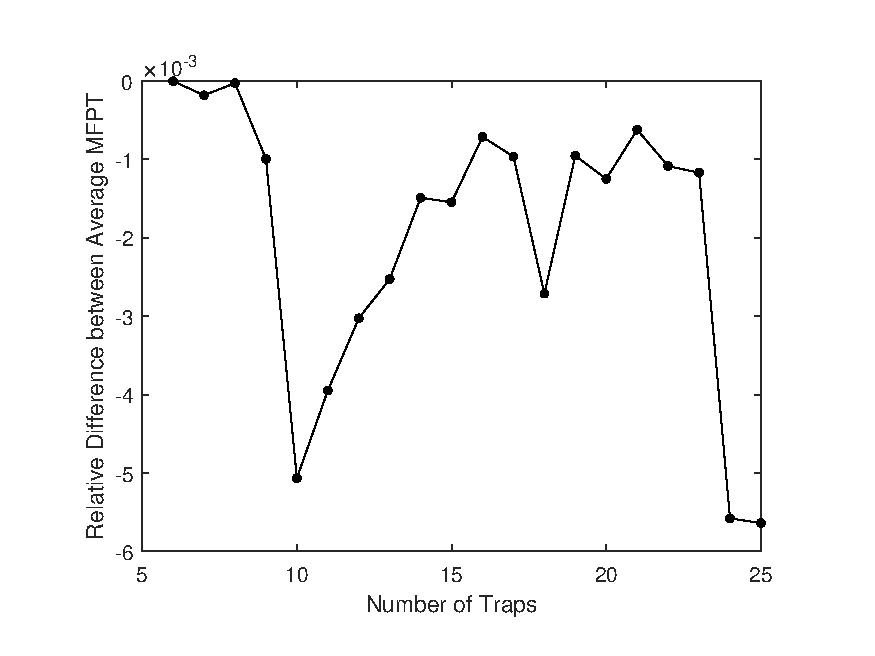
\includegraphics[width=0.5\textwidth]{RelativeDifference}
\caption{Relative difference between average MFPT in the unit disk for previously computed optimal configurations $\amfpt$, compared to that of the newly computed configurations $\amfpt'$ according to $(\amfpt' - \amfpt)/\amfpt$. Here it can be seen that the new values are consistently smaller, at most differing in the third significant figure. A table of these values can be found in Table \ref{tab:amfptComp}.}
\label{fig:amfptComp}
\end{figure}

% Merit Function
\begin{figure}[H]
\begin{subfigure}[]{
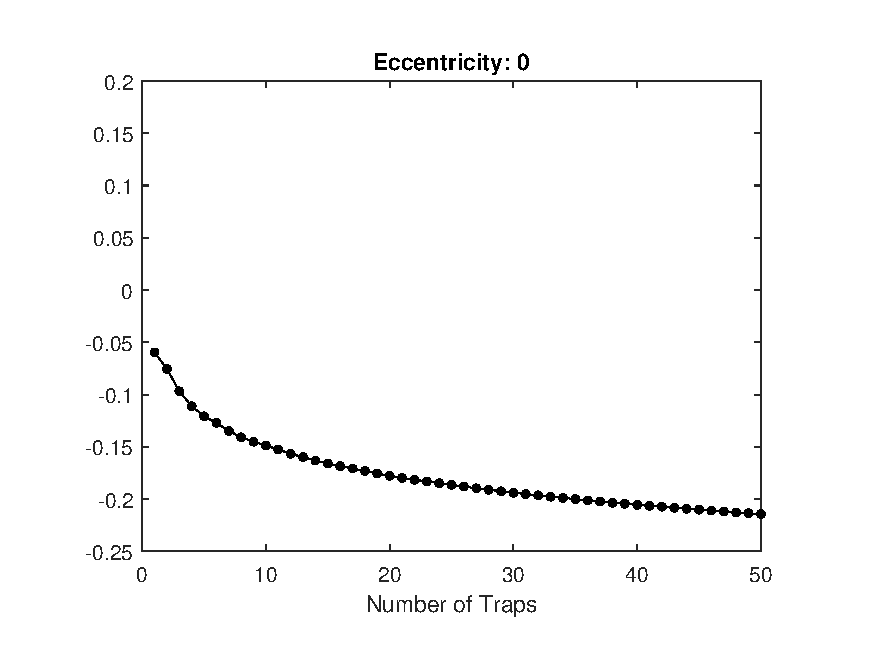
\includegraphics[width=0.5\textwidth]{MeritFunc_ecc0p0}
}
\end{subfigure}
\begin{subfigure}[]{
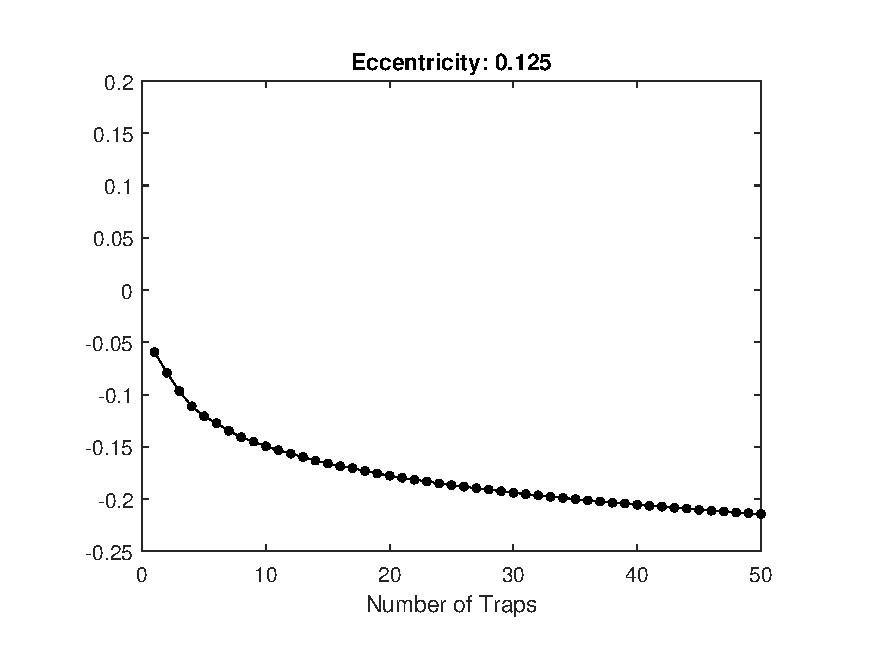
\includegraphics[width=0.5\textwidth]{MeritFunc_ecc0p125}
}
\end{subfigure}
\begin{subfigure}[]{
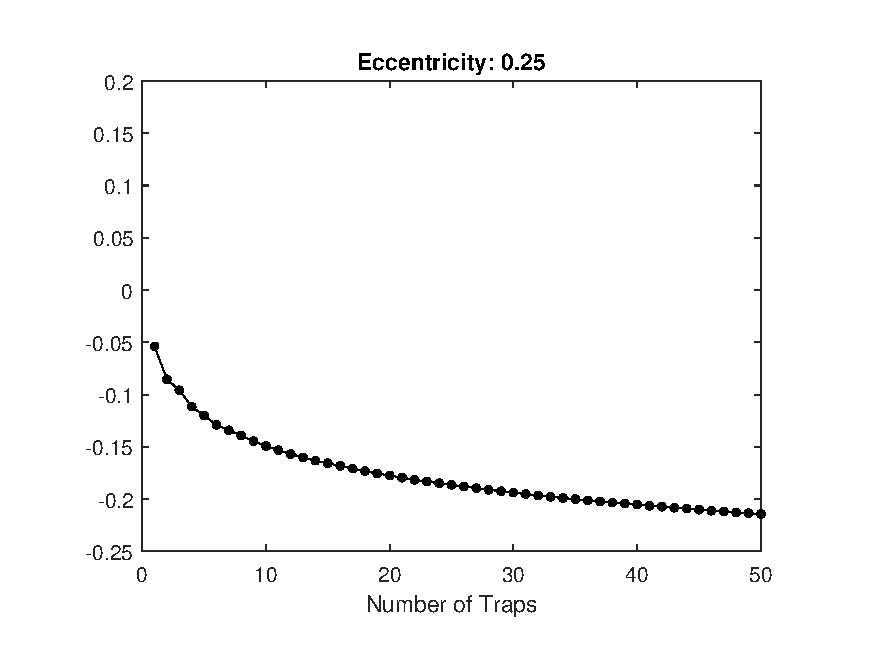
\includegraphics[width=0.5\textwidth]{MeritFunc_ecc0p250}
}
\end{subfigure}
\begin{subfigure}[]{
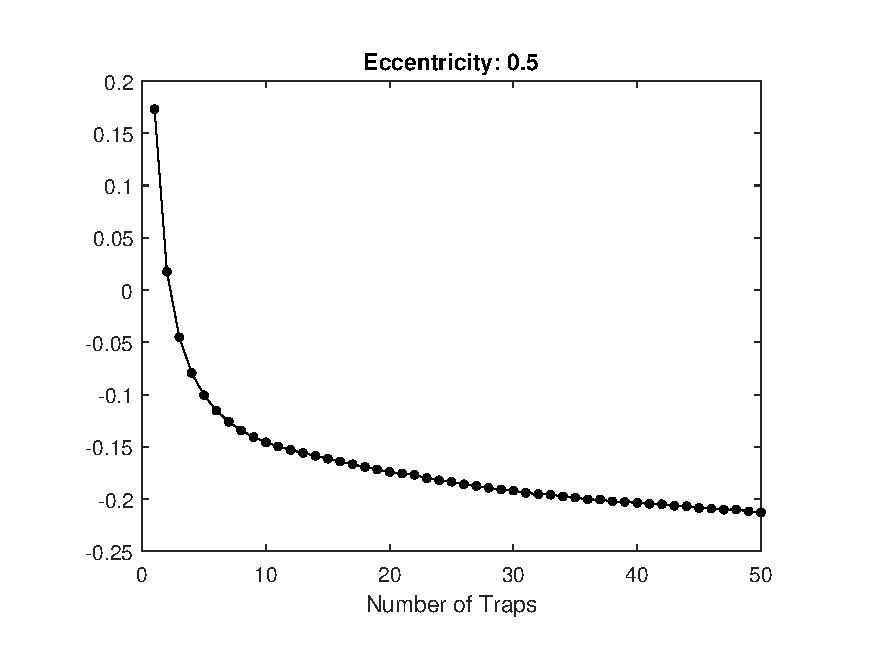
\includegraphics[width=0.5\textwidth]{MeritFunc_ecc0p500}
}
\end{subfigure}
\caption{The putative optimal values of the merit function \eqref{eq:ellMerit} for the ellipse eccentricity values
$\ecc = 0$ (a), $\ecc = 0.125$ (b), $\ecc = 0.250$ (c), and $\ecc = 0.500$ (d), as functions of the number of traps $N$. [The corresponding numerical values are presented in Table \ref{tab:meritTable}.]}
\label{fig:meritComp}
\end{figure}

% Merit function table
\newgeometry{left=2cm,right=2cm,top=2cm,bottom=2cm}
\begin{table}[H]
\begin{center}
\begin{tabular}{| c | c | c | c | c |}
\hline
$N$    & \multicolumn{4}{c|}{Merit Value} \\
  & $\ecc = 0$ & $\ecc = 0.125$ & $\ecc = 0.25$ & $\ecc = 0.5$ \\
\hline
1 & -0.0597 & -0.0594 & -0.0540 & 0.1730 \\
2 & -0.0754 & -0.0792 & -0.0854 & 0.0175 \\
3 & -0.0969 & -0.0967 & -0.0959 & -0.0452 \\
4 & -0.1112 & -0.1113 & -0.1115 & -0.0793 \\
5 & -0.1207 & -0.1207 & -0.1200 & -0.1007 \\
6 & -0.1272 & -0.1274 & -0.1289 & -0.1154 \\
7 & -0.1348 & -0.1347 & -0.1342 & -0.1261 \\
8 & -0.1409 & -0.1408 & -0.1393 & -0.1343 \\
9 & -0.1451 & -0.1451 & -0.1447 & -0.1407 \\
10 & -0.1489 & -0.1494 & -0.1492 & -0.1457 \\
11 & -0.1526 & -0.1532 & -0.1533 & -0.1498 \\
12 & -0.1567 & -0.1566 & -0.1569 & -0.1530 \\
13 & -0.1599 & -0.1598 & -0.1603 & -0.1559 \\
14 & -0.1632 & -0.1632 & -0.1632 & -0.1587 \\
15 & -0.1659 & -0.1660 & -0.1657 & -0.1614 \\
16 & -0.1685 & -0.1686 & -0.1683 & -0.1642 \\
17 & -0.1708 & -0.1705 & -0.1708 & -0.1668 \\
18 & -0.1731 & -0.1731 & -0.1733 & -0.1693 \\
19 & -0.1756 & -0.1755 & -0.1756 & -0.1718 \\
20 & -0.1777 & -0.1776 & -0.1775 & -0.1741 \\
21 & -0.1798 & -0.1797 & -0.1796 & -0.1756 \\
22 & -0.1815 & -0.1815 & -0.1816 & -0.1768 \\
23 & -0.1831 & -0.1831 & -0.1833 & -0.1800 \\
24 & -0.1848 & -0.1851 & -0.1848 & -0.1820 \\
25 & -0.1864 & -0.1867 & -0.1864 & -0.1834 \\
\hline
\end{tabular}
\begin{tabular}{| c | c | c | c | c |}
\hline
$N$    & \multicolumn{4}{c|}{Merit Value} \\
  & $\ecc = 0$ & $\ecc = 0.125$ & $\ecc = 0.25$ & $\ecc = 0.5$ \\
\hline
26 & -0.1880 & -0.1882 & -0.1880 & -0.1858 \\
27 & -0.1897 & -0.1896 & -0.1896 & -0.1875 \\
28 & -0.1911 & -0.1910 & -0.1911 & -0.1893 \\
29 & -0.1925 & -0.1925 & -0.1925 & -0.1909 \\
30 & -0.1940 & -0.1940 & -0.1938 & -0.1920 \\
31 & -0.1953 & -0.1953 & -0.1952 & -0.1941 \\
32 & -0.1964 & -0.1964 & -0.1965 & -0.1953 \\
33 & -0.1977 & -0.1978 & -0.1978 & -0.1958 \\
34 & -0.1989 & -0.1989 & -0.1990 & -0.1975 \\
35 & -0.2000 & -0.2001 & -0.2000 & -0.1987 \\
36 & -0.2012 & -0.2012 & -0.2012 & -0.2003 \\
37 & -0.2025 & -0.2024 & -0.2023 & -0.2005 \\
38 & -0.2035 & -0.2035 & -0.2033 & -0.2022 \\
39 & -0.2045 & -0.2044 & -0.2043 & -0.2028 \\
40 & -0.2056 & -0.2055 & -0.2053 & -0.2037 \\
41 & -0.2065 & -0.2065 & -0.2064 & -0.2046 \\
42 & -0.2074 & -0.2073 & -0.2073 & -0.2049 \\
43 & -0.2083 & -0.2084 & -0.2083 & -0.2065 \\
44 & -0.2093 & -0.2092 & -0.2092 & -0.2069 \\
45 & -0.2102 & -0.2103 & -0.2102 & -0.2086 \\
46 & -0.2110 & -0.2111 & -0.2111 & -0.2091 \\
47 & -0.2119 & -0.2120 & -0.2119 & -0.2102 \\
48 & -0.2127 & -0.2128 & -0.2128 & -0.2098 \\
49 & -0.2136 & -0.2136 & -0.2136 & -0.2118 \\
50 & -0.2144 & -0.2143 & -0.2143 & -0.2126 \\
\hline
\end{tabular}
\end{center}
\caption{Optimized values of the merit function \eqref{eq:ellMerit}, for each number of traps $N$ and eccentricity $\ecc$ considered in this study. Plots of these values are found in Figure \ref{fig:meritComp}.}
\label{tab:meritTable}
\end{table}
\restoregeometry



% Trap Configuration: N=5
\begin{figure}[H]
\begin{subfigure}[]{
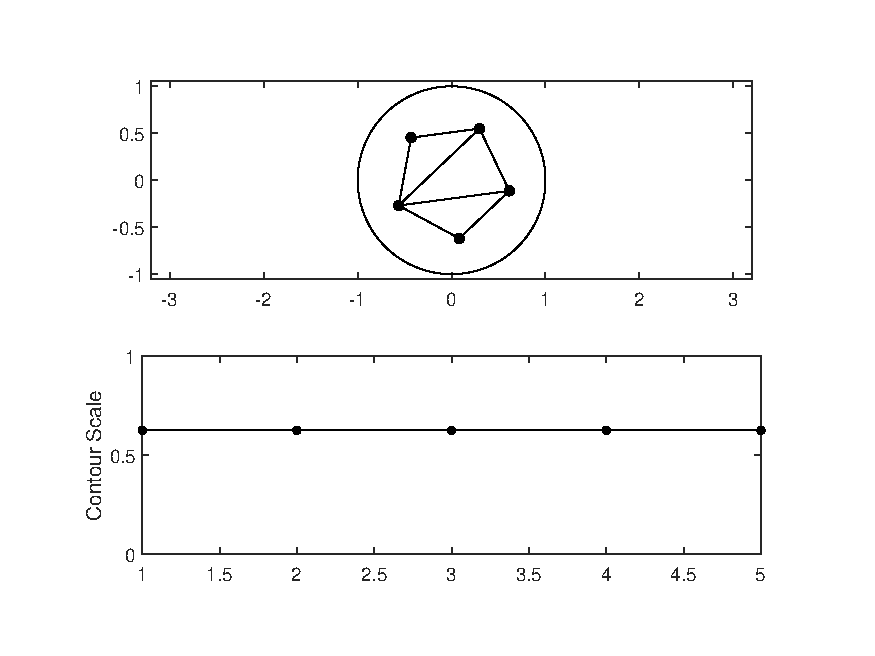
\includegraphics[width=0.5\textwidth]{TrapConfig_ecc0p0_N5}
}
\end{subfigure}
\begin{subfigure}[]{
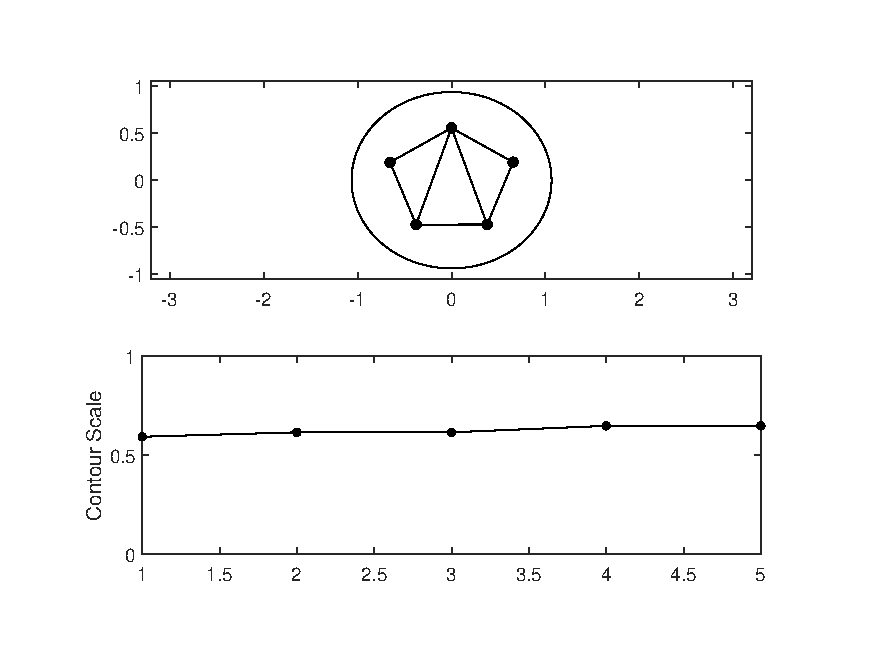
\includegraphics[width=0.5\textwidth]{TrapConfig_ecc0p125_N5}
}
\end{subfigure}
\begin{subfigure}[]{
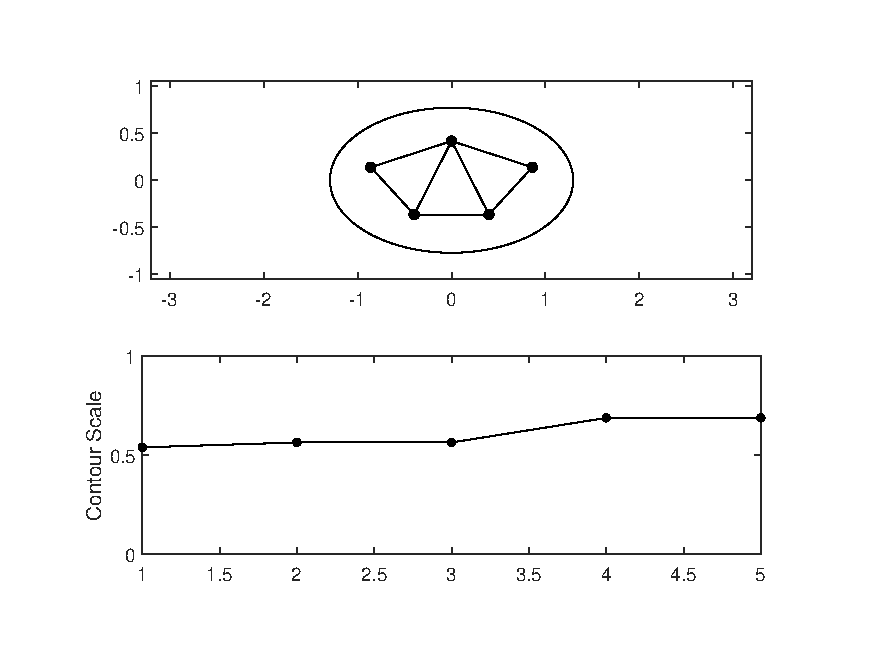
\includegraphics[width=0.5\textwidth]{TrapConfig_ecc0p250_N5}
}
\end{subfigure}
\begin{subfigure}[]{
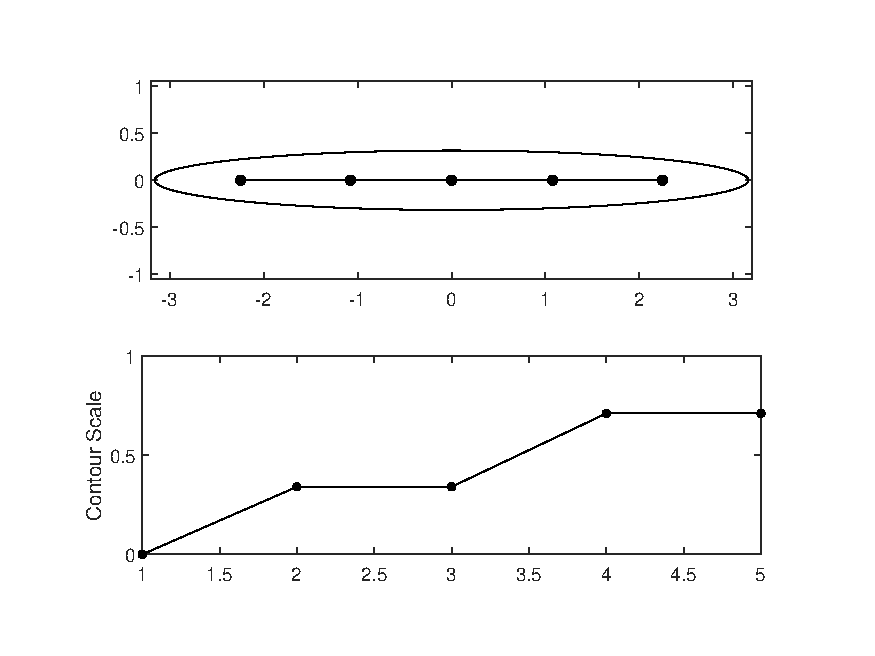
\includegraphics[width=0.5\textwidth]{TrapConfig_ecc0p500_N5}
}
\end{subfigure}
\caption{Plots depicting optimal trap distribution for $N=5$, comparing eccentricities of (a) $\ecc = 0$, (b) $\ecc = 0.125$, (c) $\ecc = 0.250$, (d) $\ecc = 0.500$. Upper plots show positions of traps along with a crude visualization of nearest-neighbour pairs calculated using Delaunay triangulation. Lower plots show the scaling factor applied to the domain boundary such that the scaled version would pass through each trap, numbered from 1 to $N$.}
\label{fig:configN5}
\end{figure}

% Trap Configuration: N=10
\begin{figure}[H]
\begin{subfigure}[]{
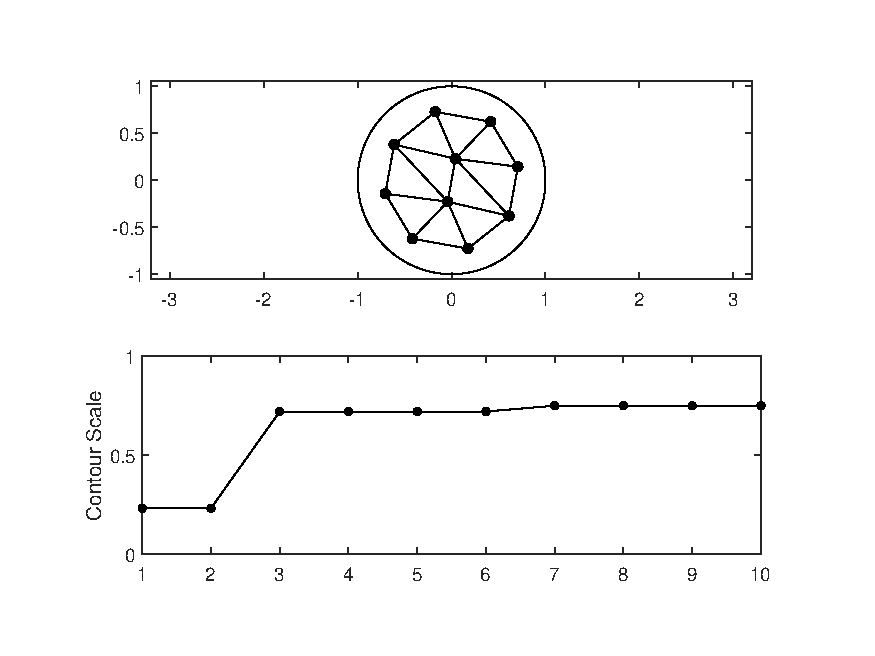
\includegraphics[width=0.5\textwidth]{TrapConfig_ecc0p0_N10}
}
\end{subfigure}
\begin{subfigure}[]{
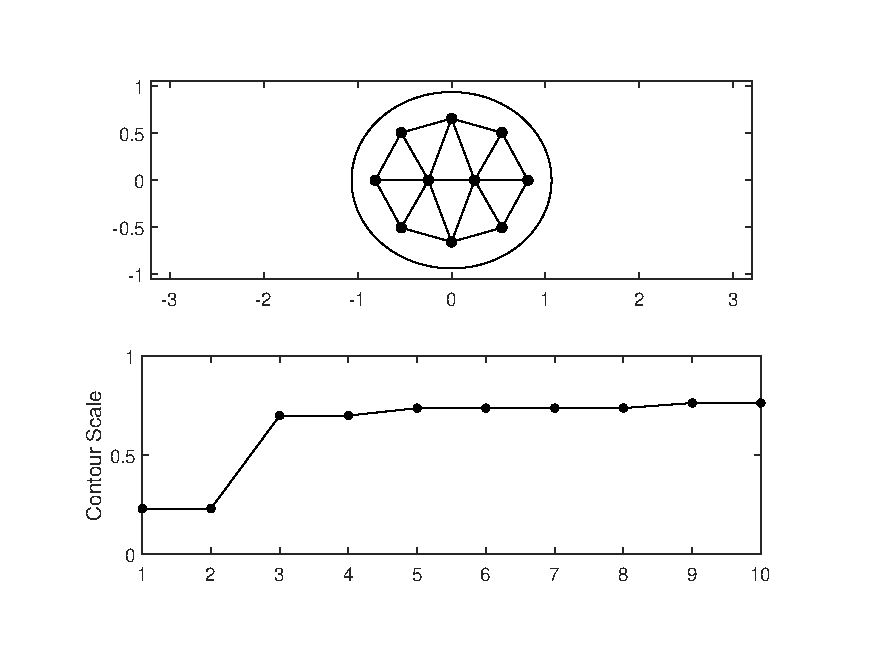
\includegraphics[width=0.5\textwidth]{TrapConfig_ecc0p125_N10}
}
\end{subfigure}
\begin{subfigure}[]{
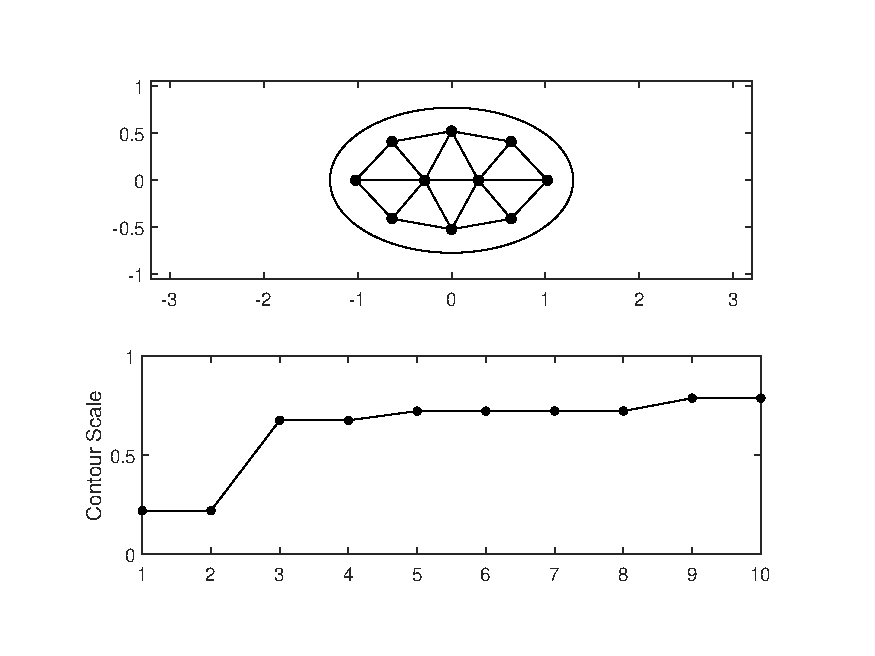
\includegraphics[width=0.5\textwidth]{TrapConfig_ecc0p250_N10}
}
\end{subfigure}
\begin{subfigure}[]{
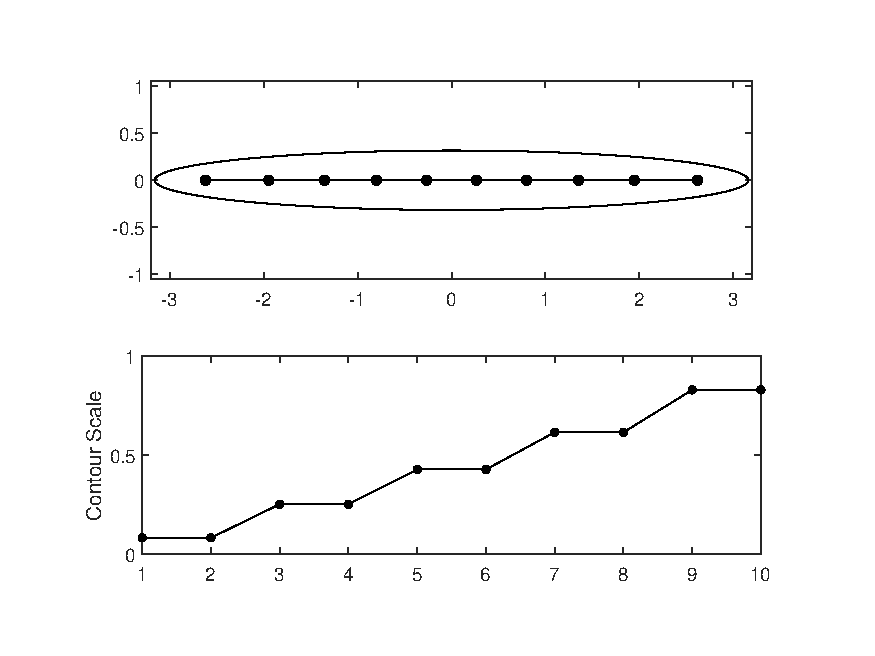
\includegraphics[width=0.5\textwidth]{TrapConfig_ecc0p500_N10}
}
\end{subfigure}
\caption{Plots depicting optimal trap distribution for $N=10$, comparing eccentricities of (a) $\ecc = 0$, (b) $\ecc = 0.125$, (c) $\ecc = 0.250$, (d) $\ecc = 0.500$. Upper plots show positions of traps along with a crude visualization of nearest-neighbour pairs calculated using Delaunay triangulation. Lower plots show the scaling factor applied to the domain boundary such that the scaled version would pass through a given trap, numbered from 1 to $N$.}
\label{fig:configN10}
\end{figure}

% Trap Configuration: N=25
\begin{figure}[H]
\begin{subfigure}[]{
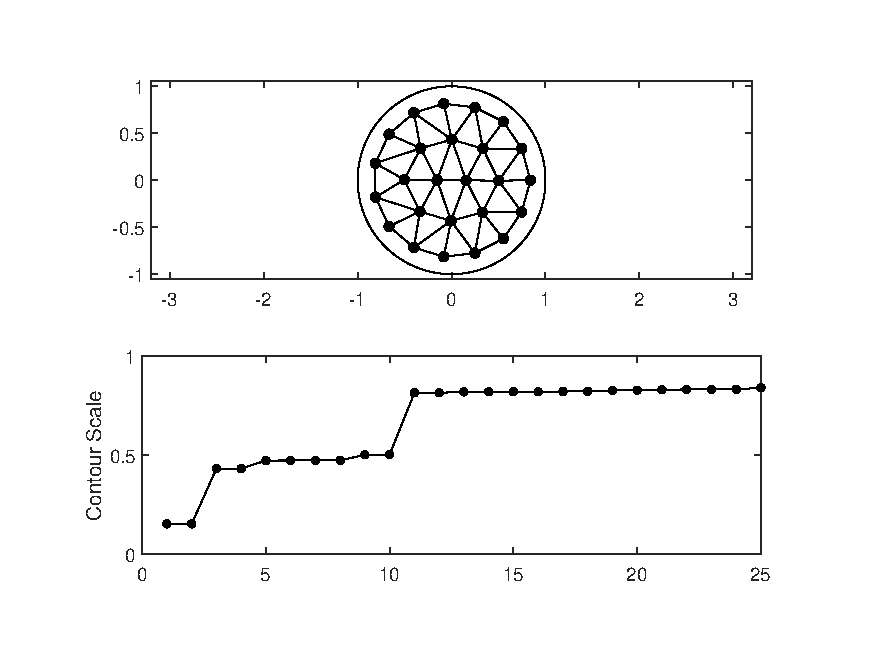
\includegraphics[width=0.5\textwidth]{TrapConfig_ecc0p0_N25}
}
\end{subfigure}
\begin{subfigure}[]{
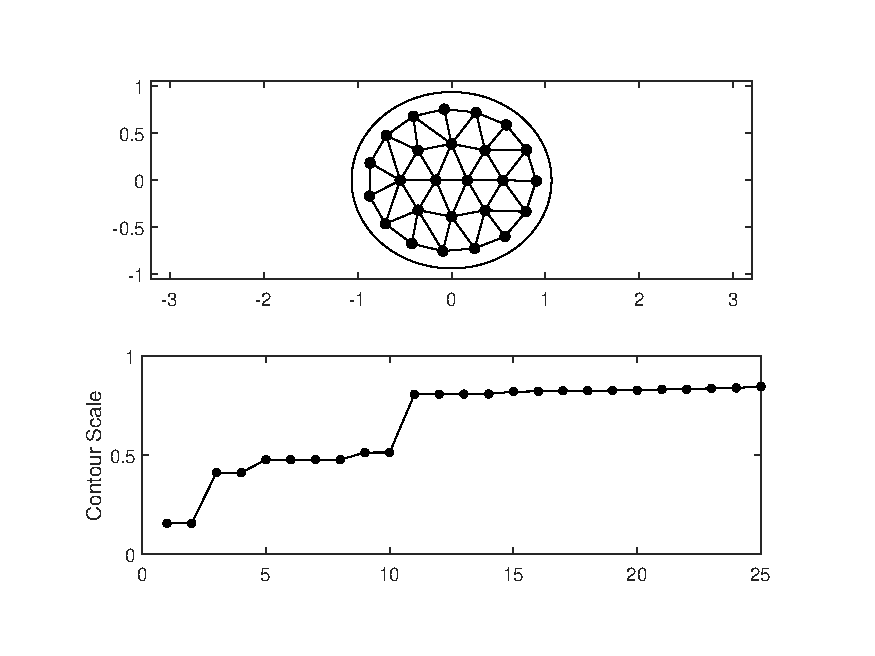
\includegraphics[width=0.5\textwidth]{TrapConfig_ecc0p125_N25}
}
\end{subfigure}
\begin{subfigure}[]{
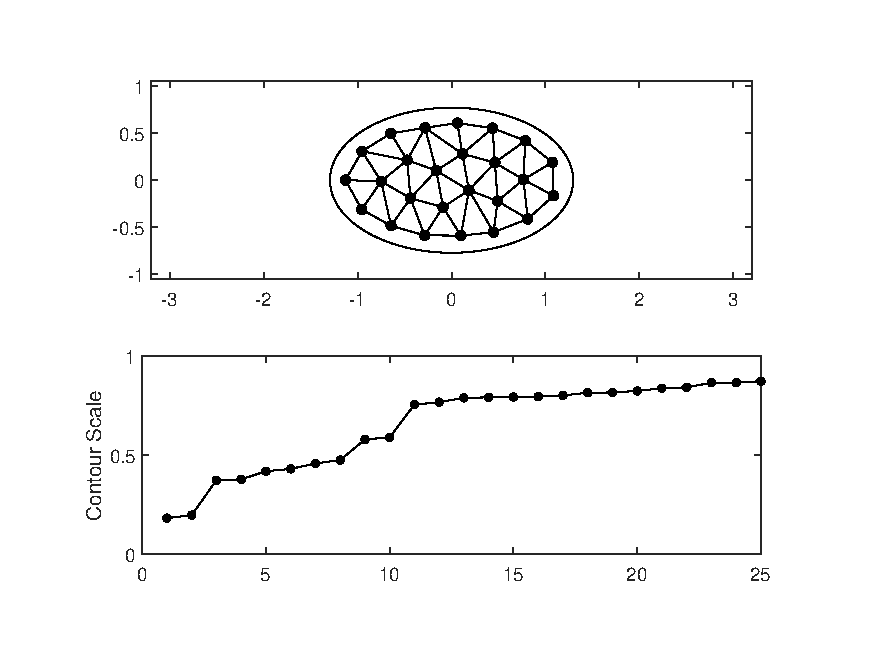
\includegraphics[width=0.5\textwidth]{TrapConfig_ecc0p250_N25}
}
\end{subfigure}
\begin{subfigure}[]{
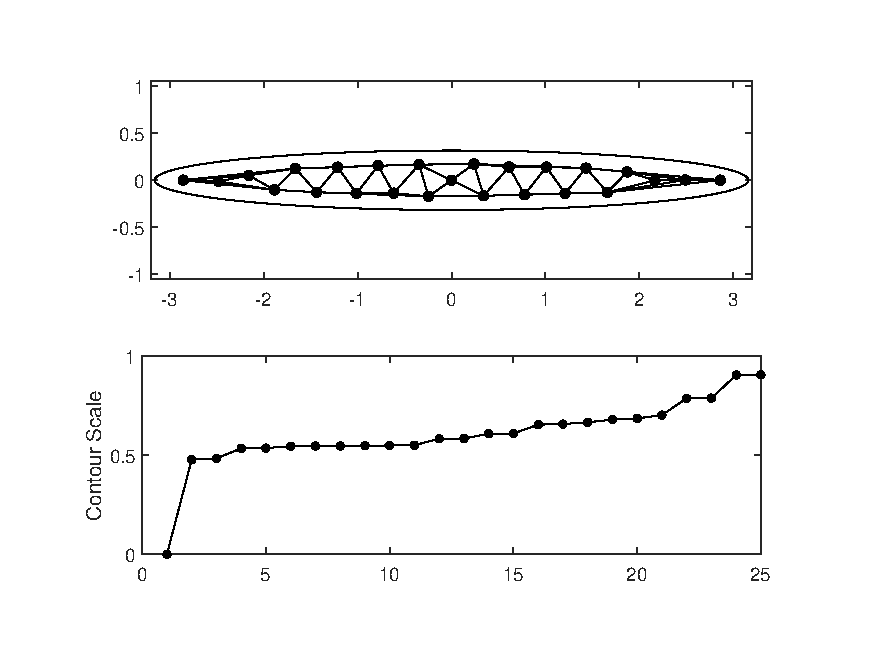
\includegraphics[width=0.5\textwidth]{TrapConfig_ecc0p500_N25}
}
\end{subfigure}
\caption{Plots depicting optimal trap distribution for $N=25$, comparing eccentricities of (a) $\ecc = 0$, (b) $\ecc = 0.125$, (c) $\ecc = 0.250$, (d) $\ecc = 0.500$. Upper plots show positions of traps along with a crude visualization of nearest-neighbour pairs calculated using Delaunay triangulation. Lower plots show the scaling factor applied to the domain boundary such that the scaled version would pass through a given trap, numbered from 1 to $N$.}
\label{fig:configN25}
\end{figure}

% Trap Configuration: N=40
\begin{figure}[H]
\begin{subfigure}[]{
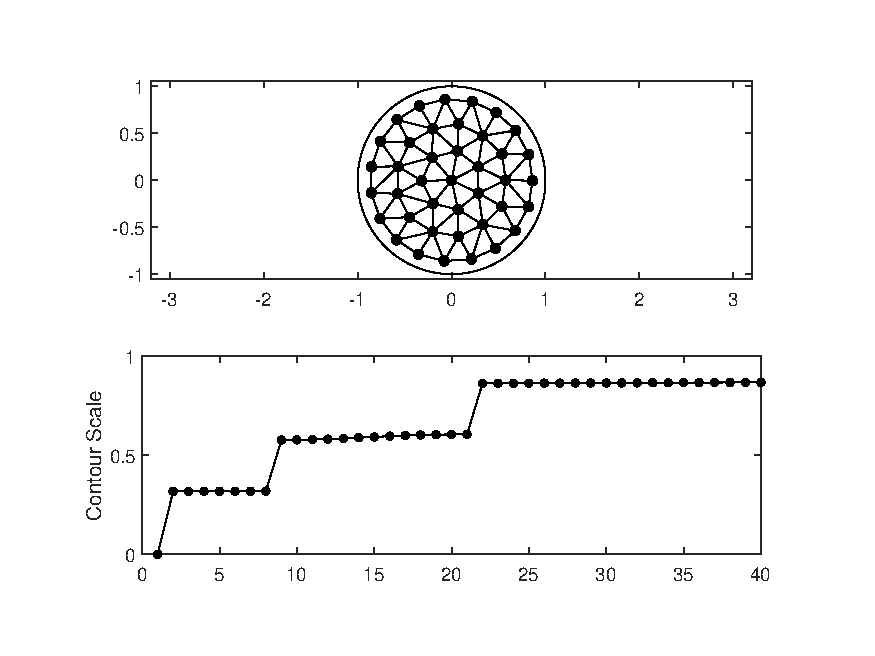
\includegraphics[width=0.5\textwidth]{TrapConfig_ecc0p0_N40}
}
\end{subfigure}
\begin{subfigure}[]{
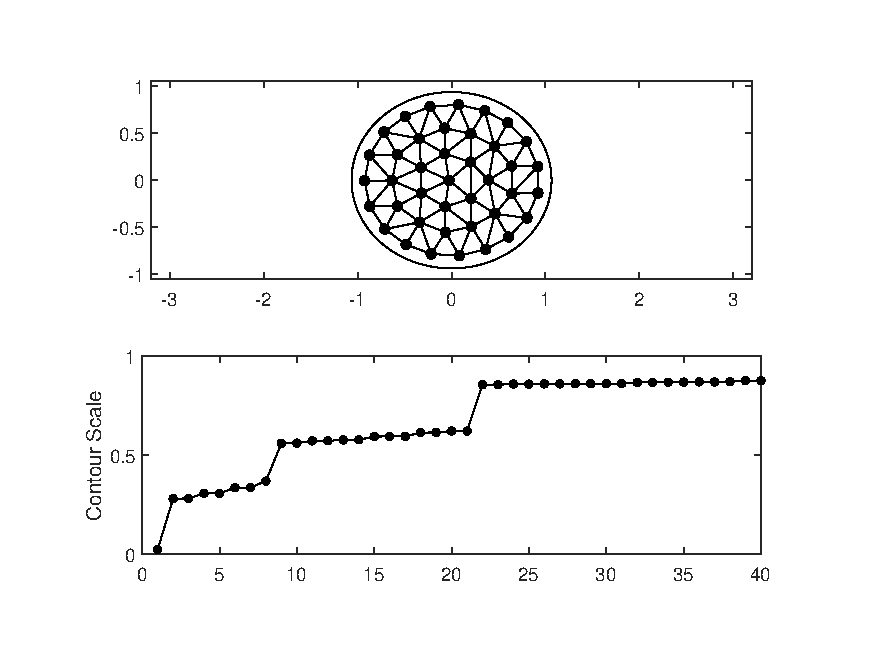
\includegraphics[width=0.5\textwidth]{TrapConfig_ecc0p125_N40}
}
\end{subfigure}
\begin{subfigure}[]{
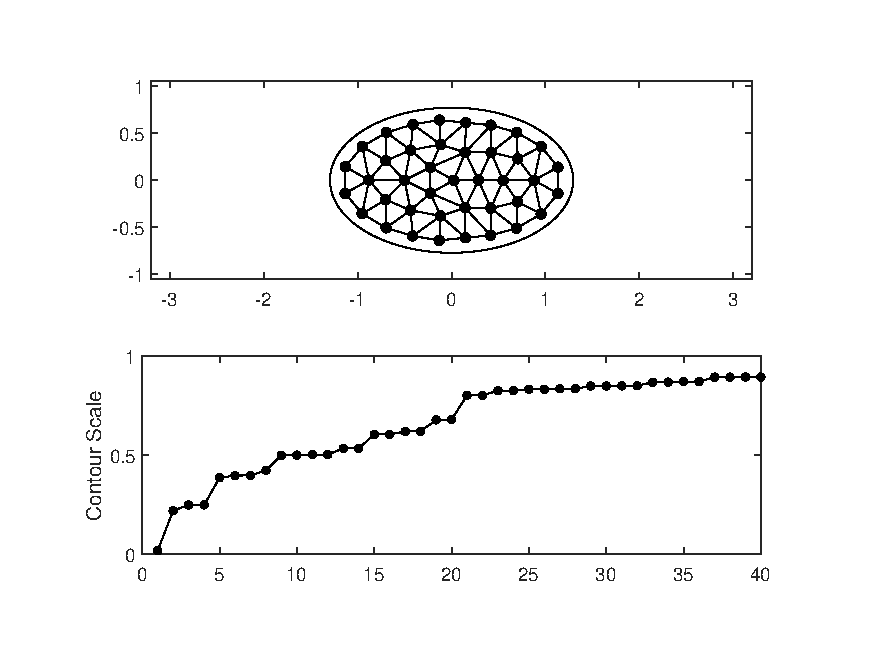
\includegraphics[width=0.5\textwidth]{TrapConfig_ecc0p250_N40}
}
\end{subfigure}
\begin{subfigure}[]{
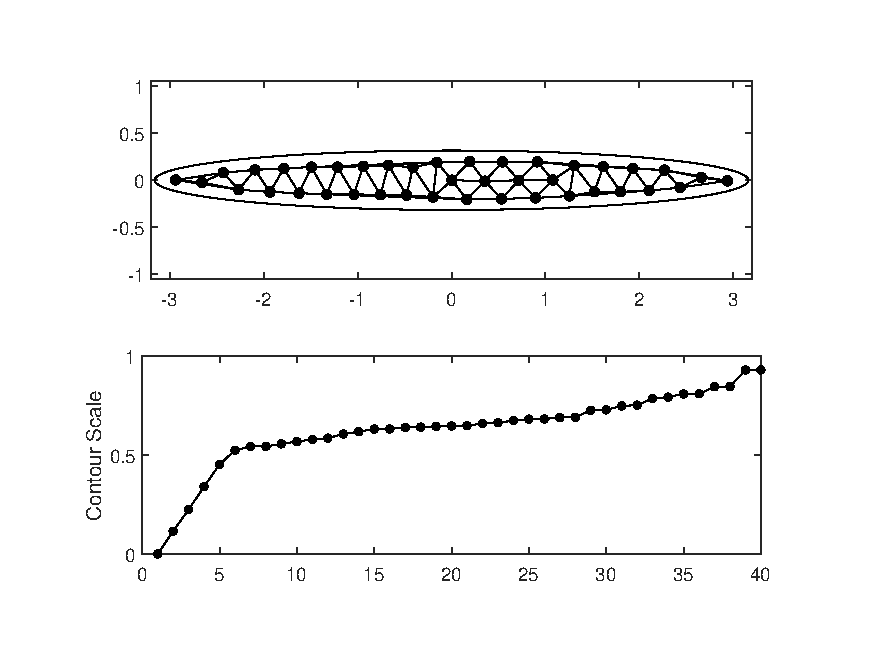
\includegraphics[width=0.5\textwidth]{TrapConfig_ecc0p500_N40}
}
\end{subfigure}
\caption{Plots depicting optimal trap distribution for $N=40$, comparing eccentricities of (a) $\ecc = 0$, (b) $\ecc = 0.125$, (c) $\ecc = 0.250$, (d) $\ecc = 0.500$. Upper plots show positions of traps along with a crude visualization of nearest-neighbour pairs calculated using Delaunay triangulation. Lower plots show the scaling factor applied to the domain boundary such that the scaled version would pass through a given trap, numbered from 1 to $N$.}
\label{fig:configN40}
\end{figure}






% Trap Distance
\begin{figure}[H]
\begin{subfigure}[]{
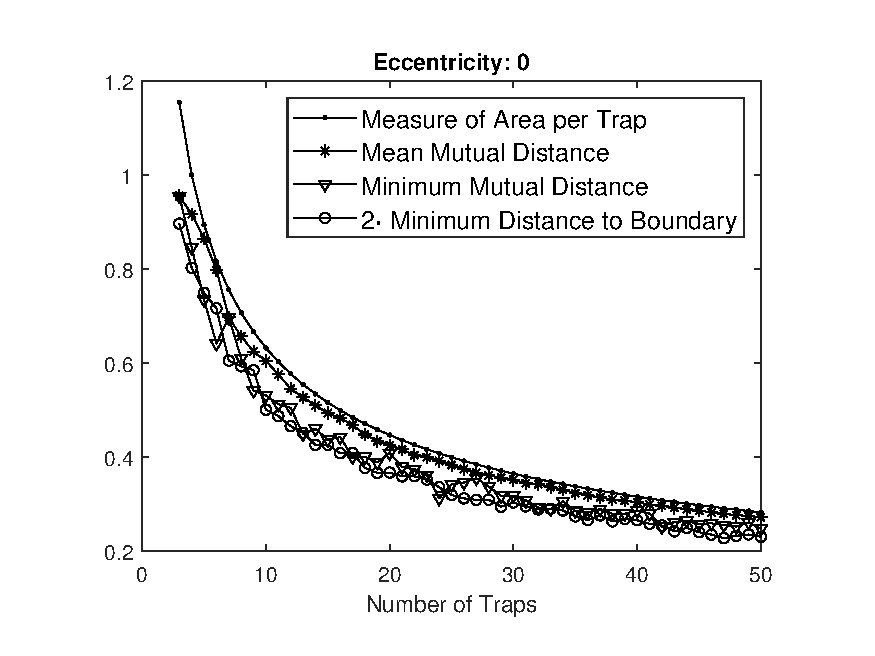
\includegraphics[width=0.5\textwidth]{TrapDist_ecc0p0}
}
\end{subfigure}
\begin{subfigure}[]{
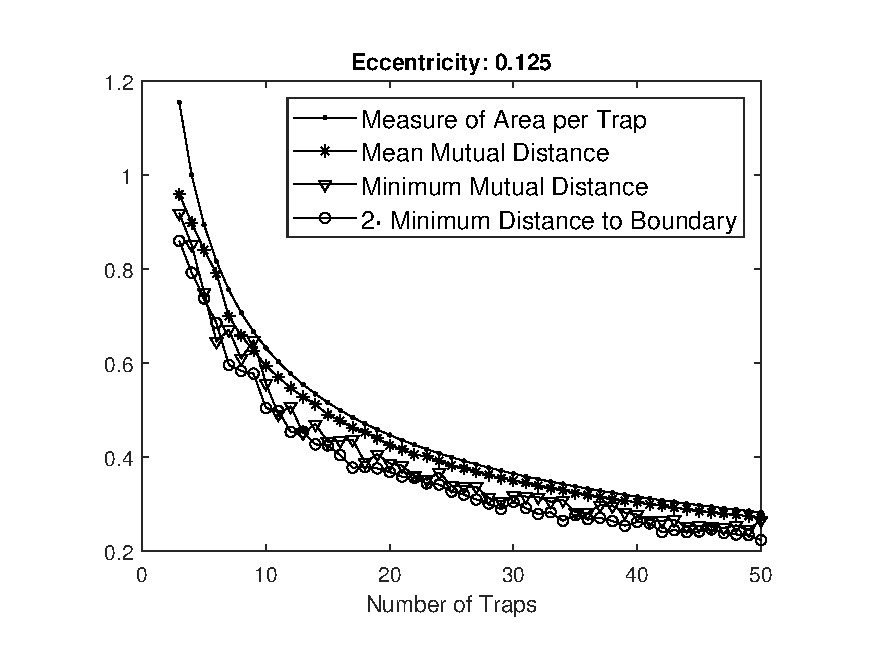
\includegraphics[width=0.5\textwidth]{TrapDist_ecc0p125}
}
\end{subfigure}
\begin{subfigure}[]{
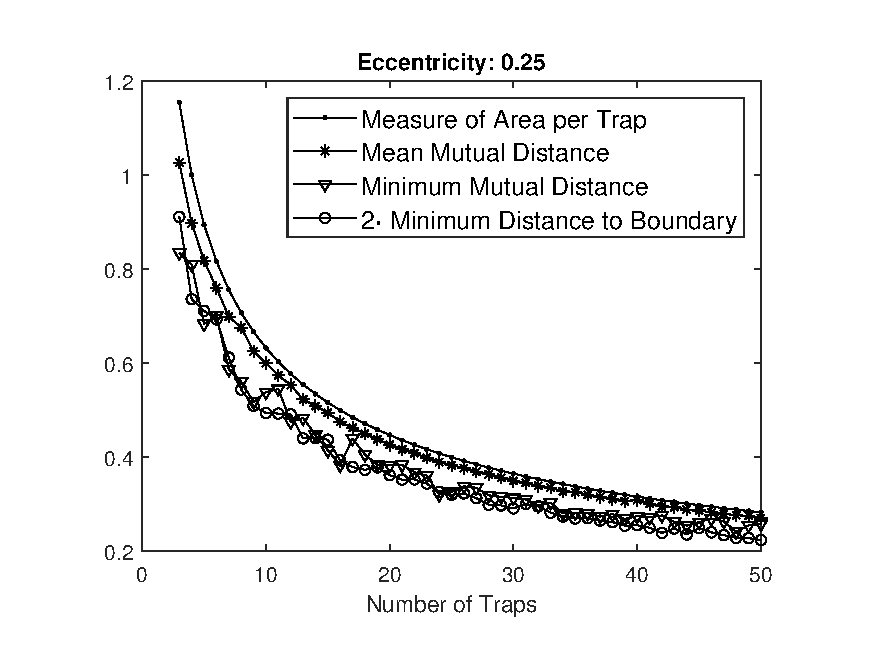
\includegraphics[width=0.5\textwidth]{TrapDist_ecc0p250}
}
\end{subfigure}
\begin{subfigure}[]{
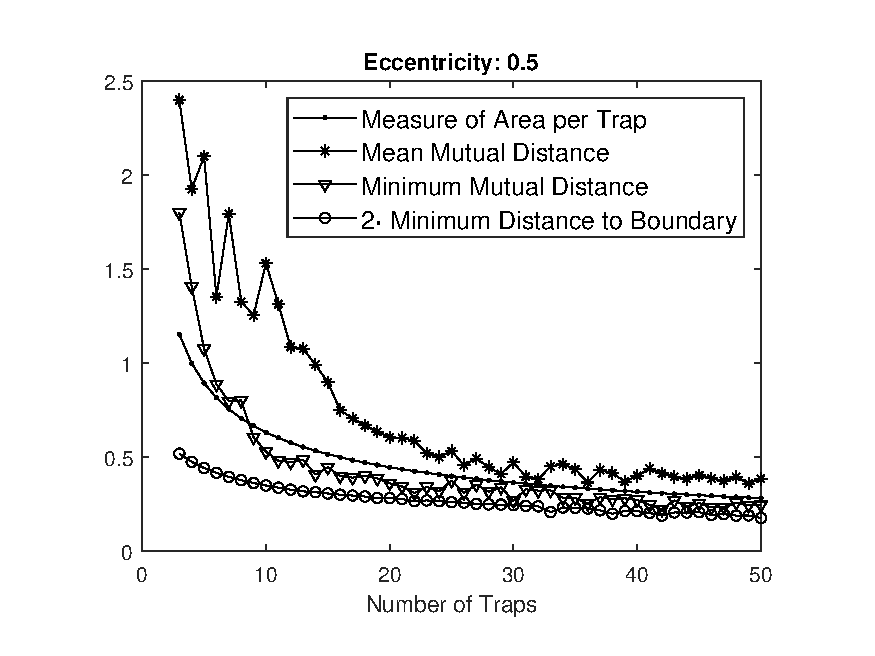
\includegraphics[width=0.5\textwidth]{TrapDist_ecc0p500}
}
\end{subfigure}
\caption{Plots depicting local properties of trap distribution, for domain eccentricities  $\ecc = 0$ (a), $\ecc = 0.125$ (b), $\ecc = 0.250$ (c), and $\ecc = 0.500$ (d). The curve entitled ``Measure of Area per Trap" shows the distance $\langle d \rangle$ computed using the ``area per trap" argument and the resulting formula \eqref{eq:avgDist}.
}
\label{fig:distComp}
\end{figure}



\section{Discussion} \label{sec:discussion}


At this point some interpretation of the previously stated results will be presented. This discussion will concern the putative optimal values of the average MFPT \eqref{eq:ellAMFPT} in elliptic domains with internal traps, values of the related merit function \eqref{eq:ellMerit}, the positions of traps within the domain, and the bulk measures of trap distribution which were employed. To begin, the method of study will be briefly reiterated. In order to study the dependence of optimal trap configurations on both the number of traps, and the eccentricity of the elliptic domain, merit functions for the average MFPT were minimized for $N \leq 50$ and eccentricity \eqref{eq:eccDef} values of 0, 0.125, 0.25, and 0.5, while the area of the ellipse was kept constant, $\domMeas = \pi$. In the search for a global optimum, an iterative approach, which switched between global and local searches, was used. The method used here was similar to that used in Ref \cite{iyaniwura2020optimization}, though a different algorithm was used for the local search, as well as in Ref \cite{gilbert2019globally} which used a different algorithm for both searches. A somewhat different approach was employed in Ref \cite{iyaniwura2019simulation}, which made use of numerical solutions to the Poisson problem.

In the case of the unit disk, comparing the results of this study to those of a previous study \cite{kolokolnikov2005optimizing} demonstrated that the optimums reported here are consistently an improvement on previous work. This is due to the use of a more accurate asymptotic expression \cite{iyaniwura2020optimization}, as well as removing the constraint that all traps be located on rings within the domain.

Plots of the putative globally optimal merit function values as functions of $N$, for each eccentricity, can be found in Figure \ref{fig:meritComp}. From these plots it seems that eccentricity is an important factor when there are few traps, around $N < 10$, but each function behaves similarly as $N$ increases. In particular, as the number of traps $N$ increases, it is natural to expect that the average MFPT $\amfpt$ \eqref{eq:ellAMFPT} approaches zero; the merit function $\meritFunc(\trapLoc)$ therefore must, as $N\to \infty$, approach from above the value $\domMeas / (4\pi^2 D\nu) \simeq -0.238$, which agrees with the plots in Figure \ref{fig:meritComp}.


Examination of the positions of traps in the optimized configurations, both visually and in terms of their radial coordinates, gives the impression that the optimal configuration is one which consists of traps placed on the vertices of nested polygons. These polygons, while irregular, seem to possess some consistent structure, including being convex. (It is interesting to note that the optimal configurations of confined interacting points often take similar forms, both in two and three dimensions \cite{sloane1995minimal, manoharan2003dense, saint2001macroscopic, hoare1971physical}.) Due to the geometrical symmetries of the ellipse, the optimal configurations are defined uniquely modulo the group $C^2\times C^2$ of reflections with respect to both axes, which includes the rotation by $\pi$. The numerical algorithms, however, choose a single specific representative of the equivalent putative globally optimal configurations. For example, for non-symmetric numerically optimal configuration, several traps may be found along the midline of one half (right or left) of the domain. Optimal trap configurations with the same symmetry group as the ellipse were also observed (see, e.g., Figure~\ref{fig:configN10}(c)).


In addition to the examination of individual trap positions in each optimized configuration, quantities were calculated using the distances between neighbouring traps, defined according to a Delaunay triangulation of the trap coordinates, which served as bulk measures of the distribution of traps in each configuration. Plots of these measures, shown in Figure \ref{fig:distComp}, illustrate that the mean distance between neighbouring traps tends to be close to the diameter of a circle which would occupy the average area of the domain per trap, as in equation \eqref{eq:avgDist}. Additionally, the minimum distance between any two traps tends to be twice the minimum distance between a trap and the domain boundary, which supports the intuitive reasoning that for the boundary value problem \eqref{eq:defPDE} with interior traps, the Neumann boundary condition on $\partial\Omega$ ``reflects" each trap, so that under the average MFPT optimization, every trap tends to ``repel" from its reflection in the boundary the same way as it is repelled from other traps.

In future work, it would be of interest to address two related problems. The first is to carry out similar investigations for the near-disk domains considered in Ref.~\cite{iyaniwura2020optimization}. Another interesting direction is the development of a scaling law which would predict the behaviour of the MFPT as the number of traps increases with their positions defined according to a specific distribution, in particular, for distributions that globally or locally minimize MFPT, or other distributions of practical significance. A similar problem, along with the dilute trap fraction limit of homogenization theory, was addressed in Refs.~\cite{cheviakov2010asymptotic, cheviakov2013narrow} for the narrow escape problem involving boundary traps located on the surface of a sphere in three dimensions.

\subsection*{Acknowledgements}
A.C. is thankful to NSERC of Canada for research support through the Discovery grant RGPIN-2019-05570.


\bibliography{BibList7d}
\bibliographystyle{unsrt}



\end{document} 